\documentclass[12pt]{article}
\usepackage[letterpaper,portrait,margin=1.0in]{geometry}
%

\usepackage{longtable}
% begin fonts section
% for use with xelatex and lualatex but not with pdflatex
\usepackage{fontspec}
\usepackage{times}
\setmainfont{times}
% comment or uncomment AMS math symbol as needed
\usepackage{amssymb}
% comment or uncomment and use other Greek packages as needed  
\usepackage{textgreek} % use in textmode (bibliographies), non-italicized upright non-bold font
\usepackage{upgreek} % use in mathmode (equations), non-italicized upright bold font
% end fonts section
\usepackage{grffile}
% begin other packages section
\usepackage{setspace}
\usepackage{fancyhdr}
\usepackage[svgnames]{xcolor}
\usepackage{url}
\usepackage{nameref}
\usepackage[colorlinks=true,linkcolor=blue,citecolor=blue,urlcolor=blue]{hyperref}
\usepackage{algorithmicx}
\usepackage{graphicx}
%\usepackage{rotating}
%\usepackage[justification=centering]{caption} 
% end other packages section
\usepackage{wrapfig}

% begin BibLaTeX section
\usepackage[backend=biber,texencoding=utf8,bibencoding=utf8,style=ieee,maxnames=3,bibwarn=true]{biblatex}
\renewcommand*{\revsdnamepunct}{} % to eliminate the extra comma between last name and firstmiddle initials
% remember to include the *.bib extension on filenames in the \addbibresource{BibliographicResourceFile} command
%\addbibresource{CarlTaswell.bib}
\addbibresource{JSHS_bibliography.bib}
% http://tex.stackexchange.com/questions/121661/biblatex-remove-the-eng-from-citations
\AtEveryBibitem{\clearlist{language}} % removes unnecessary use of "eng" as language
% https://tex.stackexchange.com/questions/331870/is-there-a-recommended-way-to-replace-cite-with-parencite
\AtBeginBibliography{\small}
% end BibLaTeX section
\usepackage{multirow}

% local macros for LaTeX document
% additional preamble with commands, example custom hyphenation, and header declarations
\newcommand{\BibLaTeX}{Bib\LaTeX}
\newcommand{\etal}{\textit{et al}.}
\newcommand{\pdscod}[1]{\textbf{#1}}
\newcommand{\regtm}{\textsuperscript{\textregistered}}
\hyphenation{non-dis-cri-mi-na-tion tele-gaming TeX-studio}
\setcounter{secnumdepth}{3}
%\nocite{*}
\begin{document}
	\thispagestyle{empty}
	\begin{center}
	
	{\LARGE SHIRASE: Automated Construction and Analysis of Semantic Graphs Derived From Open-Web Resources for a Hybrid Lexical-Semantic Search Engine}
	\vspace{8mm}
	
	{\Large Shiladitya Dutta}
	\vspace{8mm}
	
	{\Large Foothill High School}
	\vspace{5mm}
	
	{\large 4375 Foothill Rd, Pleasanton, CA 94588}
	\vspace{20mm}
	
	{\large January 18th, 2019}
	\end{center}
    \pagebreak
    %-----------------------------------------------------------------------
    {\Large Acknowledgments}
    
    \vspace{3mm}
    \noindent
    I would like to acknowledge Foothill High School and Shannon Sos for helping me develop this project along with facilitating my participation in JSHS.
	\tableofcontents
	\thispagestyle{empty}
	\pagebreak
    \setcounter{page}{1}
	\section{Introduction:}
	\subsection{The Current State of the Internet}
	\quad Currently, the internet is heavily lexically based. This means that it is based on the syntactic structure of words in a particular document rather than the meaning of the information being stored on the document itself. On an implementation level, this translates to data being stored on the web in such a way that computers, unless they use a form of metadata attached to an article (i.e. tags, categories, keywords, etc.), cannot understand the data that they are accessing. Because of this, search systems have to depend on the lexical structure of the data to interpret the articles that the user wants to retrieve, thus leading to the prevalence of keyword matching search engines which attempt to match phrases or words from a user’s query with key phrases or words from a particular web page of interest. Though these can be effective in interpreting the intent of a user in many scenarios, it is still nevertheless lacking in that the computer understands neither the information it is processing nor the query that the user has given. Thus, current search engines are designed to look for resources that may contain the answer to the user’s query rather than directly answering the question. Thus, these search engines can only look at resources individually, and are unable to incorporate information from multiple resources since they cannot understand the information in those resources in the first place. This impedes the specificity and versatility of the searches that the user can make, since the search can only access information from one data source at a time, thus meaning that complex searches which necessitate multiple resources are impossible. In addition, search queries that involve specific information are troublesome to conduct, since the search engine cannot interpret data from the resources other than looking at the syntactic structure. For example, a user would be hard pressed to find “Famous Chemists born in Birmingham before 1874”, since even though this information would be present on disparate sources on the internet, such as individual information pages on English chemists, it is unlikely that there would be a singular page that would contain the answer to such a specific question.
	\subsection{The Semantic Web}
	\quad This is where semantic web technology, also known as Web 3.0, comes into play \cite{berners2001semantic}. Web 3.0 represents a paradigm shift in the way online data is stored and processed. Rather than relying on the lexical data stored on individual documents, the semantic web is based on linked data/semantic graphs aggregated from a variety of resources. By cutting out the middleman between relevant information and the user, it is far more intuitive to perform queries, since information from a variety of resources is represented directly on a unified linked data graph, thus allowing a semantic search system to interpolate data from a wide variety of resources to answer a single query. The semantic web is able to do this by representing facts and statements on a graph using the Resource Description Framework (RDF) format \cite{lassila1999resource}. The RDF data format renders linked data via a series of RDF triples. A single RDF triple consists of a subject, verb, and object, acting in a manner analogous to a line segments as two nodes (the subject and object) and a line (the verb). The subject is used to represent the target entity, the verb represents a characteristic or aspect about the subject, and the object represents the value or target of the verb. Each of these triples is used to represent a particular statement. For example, to say that “Bobby is 42 years old”, the triple would be: Bobby, Age, 42. Each segment of these triples is represented by an Unique Resource Identifier (URI), which is similar in structure to an URL, but is used to denote specific entities or concepts rather than webpages \cite{berners2004uniform}. Combinations of these RDF triples can be made to create a graph that can describe and connect a multitude of entities. However, a repository of information is relatively useless without a method to search and analyze it. As such, there is SPARQL Protocol and RDF Query Language (SPARQL) \cite{harris2013sparql}. SPARQL, as suggested in the acronym, is a query language used to interact with RDF. SPARQL is based on the use of a series of conditions in order to create searches.  Due to the fact that information is explicitly represented on the graph, users can make complex composite search queries that have a variety of conditions and that return a wide range of information back to the user. This can be anything from the provenance of the answers if they are searching for general web pages, to answering specific questions such as birth dates or population numbers. In addition, the graph-like nature of the data format allows for search engines to integrate multiple triples to create new connections between nodes, such as one triple saying that “humans are mammals” and another triple saying that “mammals are animals” could be used to form the connection that “humans are animals”.
	\subsection{The Problem With the Semantic Web}	
	\quad Even though Web 3.0 has so many advantages over Web 2.0, it has yet to hit the mainstream in spite of the idea being around for at least a decade. The reason is that, while the semantic web brings some incredible benefits, it also has a few crippling drawbacks. This project attempts to ameliorate two of these drawbacks: the high upfront investment required to create a viable semantic graph and relative unusability of the current search methods. Most semantic graphs require a massive labor and time investment to generate. This is because the current method of building semantic markup, barring graphs where the main purpose is to act as a supplement to the lexical content by already known metadata, depends on manual curation. This leads to a high upfront cost that acts as a hard barrier to many ventures into the area along with discouraging companies from open-sourcing their networks The second issue is that the search method for the semantic web is relatively unapproachable. Currently, most semantic graphs can only be queried via SPARQL, or some other form of related query language. For obvious reasons, learning a query language is daunting to an average user, making it so that the only real users of many semantic databases are other software programs which use the database to supplement their own service. In line with this, most semantic databases present today (i.e. Google Knowledge Graph) are used to supplement existing lexical utilities. In the case of Google Knowledge Graph, it is used to give answers to questions which ask for a specific fact, such as “How long is the Mississippi?”. Even though most companies such as Google, Facebook, Twitter, and even Best Buy have built their own linked data networks, these networks are tailored to specific applications, and meant to act as supporting structures rather than primary applications. 
	\subsection{Overview of Solution}
	\quad These two problems are proposed to be solved via the implementation of a hybrid lexical-semantic search engine: SHIRASE. The Semantic-lexical Hybrid Information Retrieval And Search Engine(SHIRASE) works by dynamically pulling information from select literature databases based on a user's search and converting information from the open web to semantic records. SHIRASE is then able to search those records, along with all previously converted records, for the requested information. This pipeline allows for the gradual accumulation of converted semantic records, meaning that over time as more searches are performed, the pool of information to search within will become larger. This provides a solution to the problem of the high time investment required for linked data creation since the process is automated and gradual thus allowing for the graph to grow over time. This avoids the issue of having an immensely large initial runtime for the linked data graph creation. To solve the problem of the unapproachability of the SPARQL search method, a SPARQL builder form has been created which would build the SPARQL queries for a user. The main feature of the semantic search engine is that it doesn’t just search for articles, it can also just return specific features of articles, which can be useful for users who want to get specific information from articles without having to read each article (such as the spacing for multi-modal scans used by studies on neurodegenerative diseases). Currently, SHIRASE has been specifically applied to searching through research literature, but SHIRASE's framework can be generalized to a variety of other content. With this system, an end-to-end implementation solution for semantic search is delivered to the user, allowing for the gradual conversion of open-web resources to an unified semantic graph while at the same time offering a far more versatile search method than any other traditional search engines.
	
	\section{Methods}
	
	\quad SHIRASE has 4 main sections: the web crawler, the lexical-to-semantic converter, the triplestore, and the internal search engine. The web crawler retrieves articles from the open-web using the user provided general search query. The lexical-to-semantic converter takes the text of the article and translates it into an RDF linked data graph representing the text. These graphs are then stored in the triple store which can be searched using the Internal Search Engine. These 4 sections work in unison to create an end-to-end search semantic search engine.
	\begin{figure*}[h!]
		\centering
		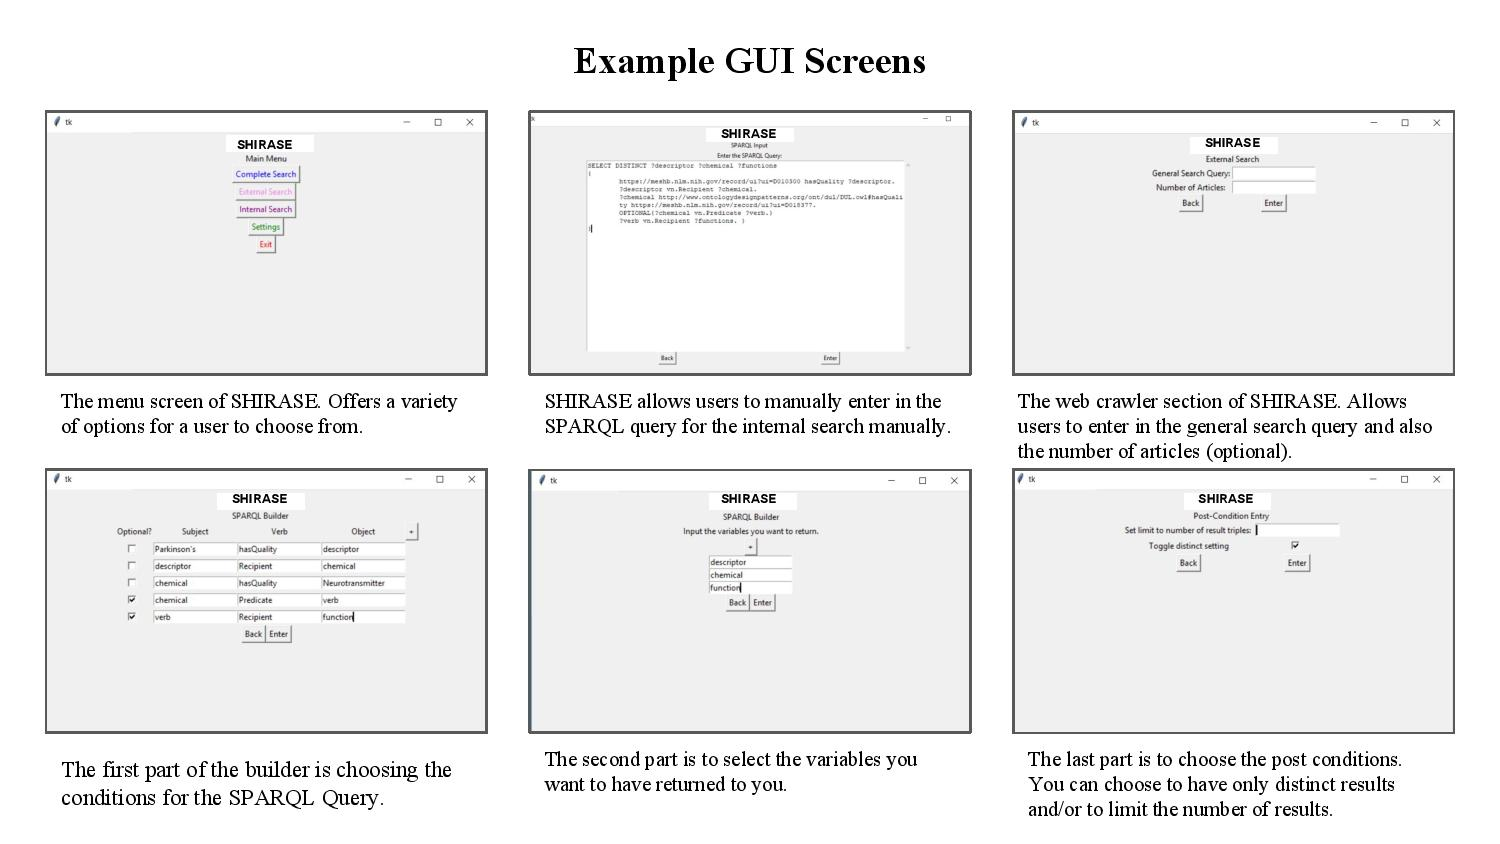
\includegraphics[scale=0.67]{ExampleGUIScreens}
	\end{figure*}
	The interface of SHIRASE can either be the Command Line Interface or a graphical user interface. The user can either do a complete search, an external search, or an internal search. The external search is a search that converts more articles into semantic graphs to expand the reach of the internal search engine. The internal search is a search in which the user searches through the articles that have already been converted into linked data. The complete search is a combination of the internal and external search where the system converts articles from the open-web and then searches through the converted and all previously converted articles. The external search should be used when the user just wants to add converted articles to the store. The internal search is used when the user is confident that the articles that they have already converted adequately describe their target search area. The complete search is used when the user wants to perform a search where the target search area isn’t adequately covered or simply to ensure that every possible article of interest is searched. 
	\begin{figure*}[h!]
		\centering
		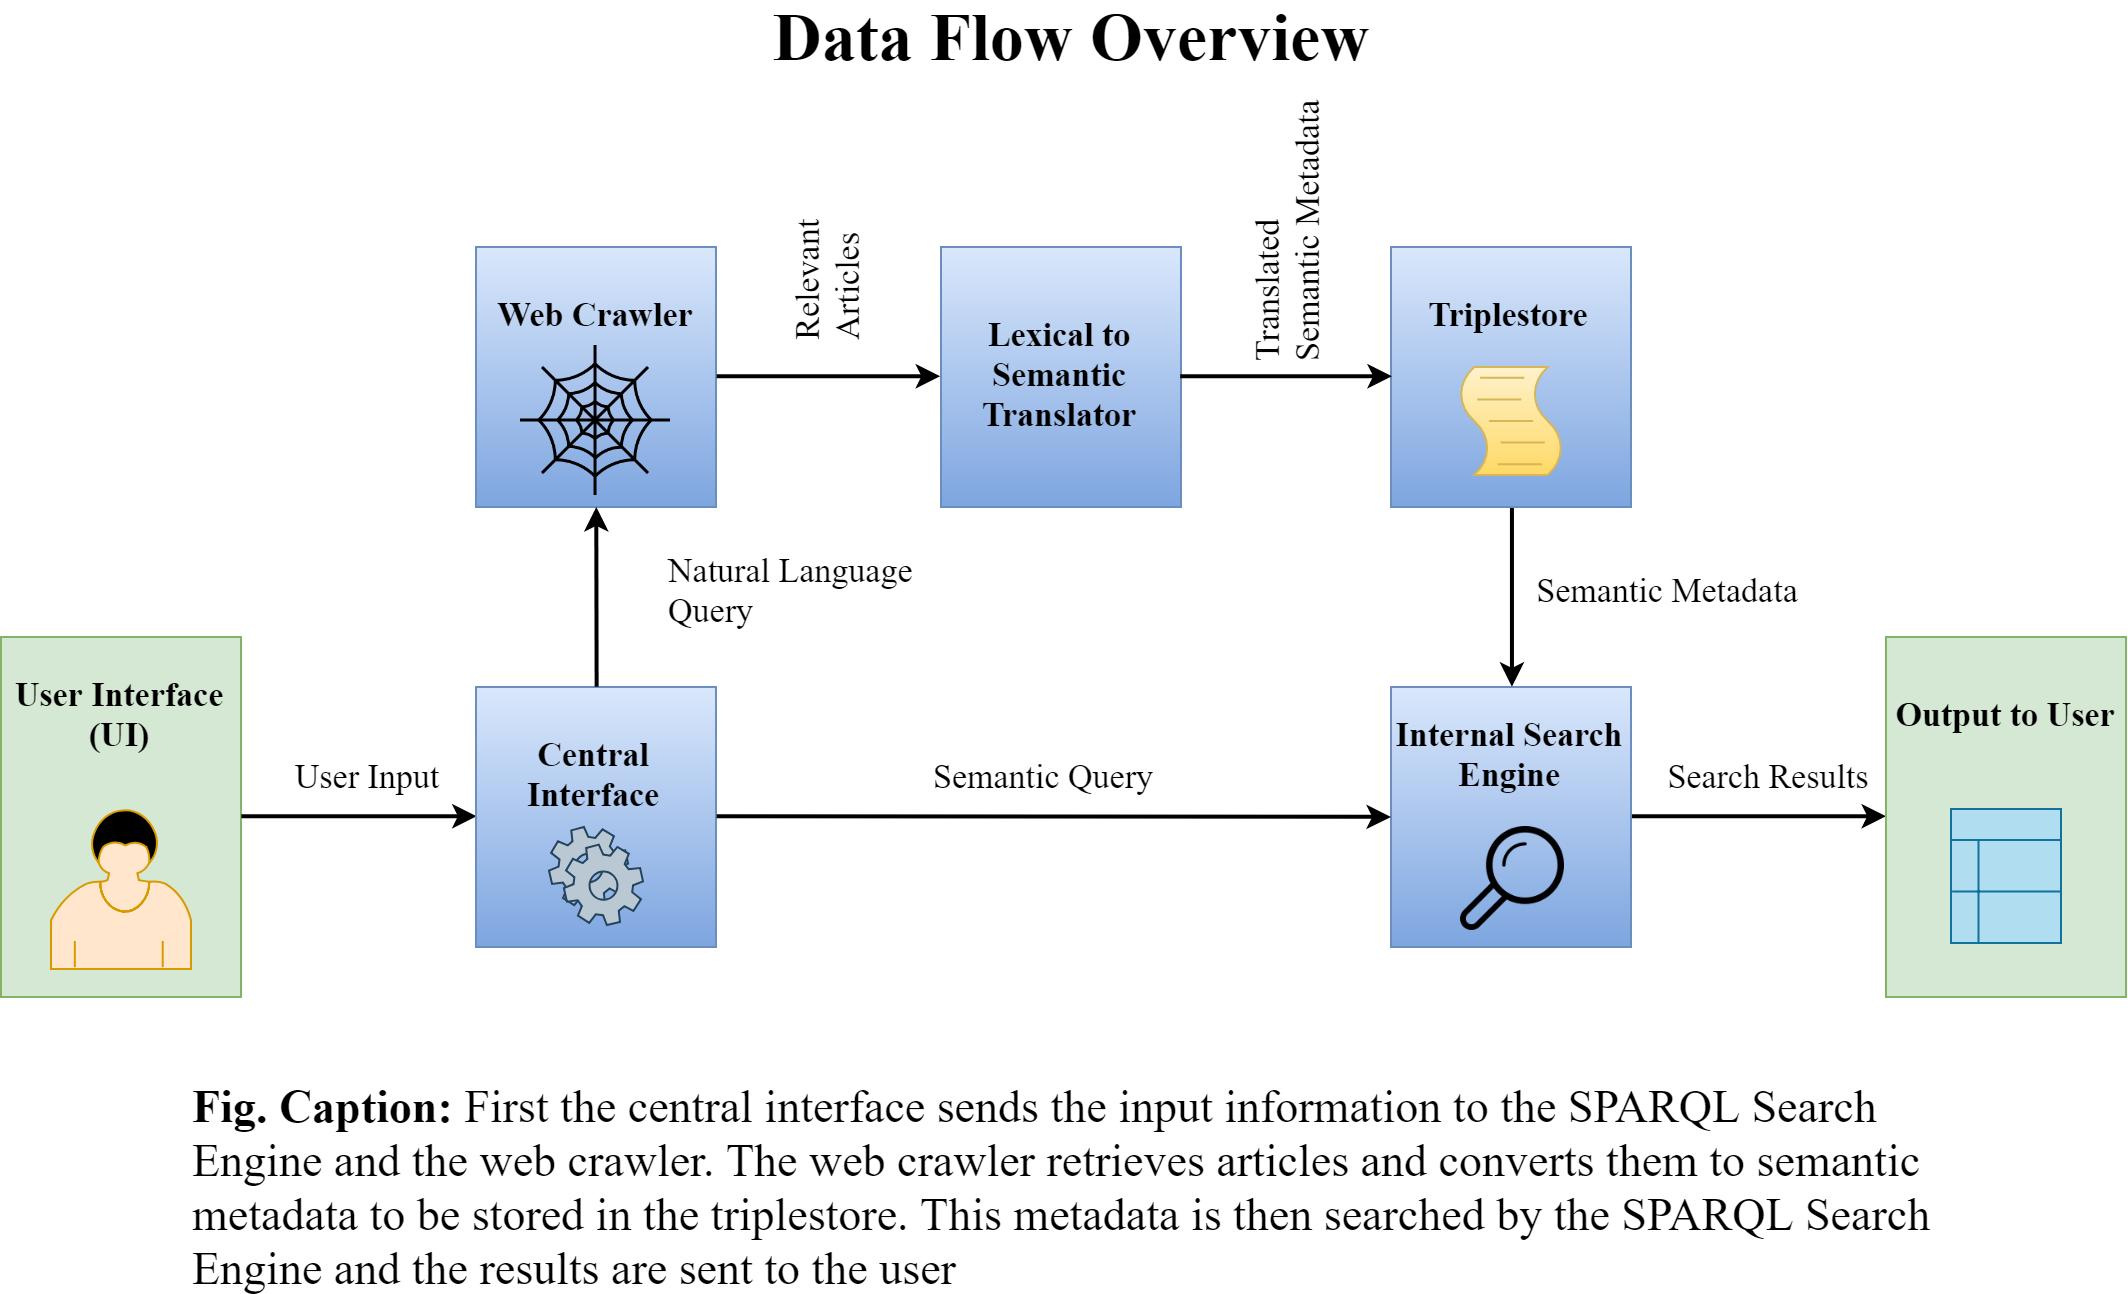
\includegraphics[scale=0.21]{GeneralDiagram_vJSHS2.0}
	\end{figure*}
	For the external search the user inputs the general search query. If necessary, a user can specify the number of articles they want to retrieve. For the internal search, the user inputs a semantic query. The builder form allows the user to input a semantic query without having to know SPARQL syntax. The user can also input a SPARQL query directly if they so choose. The input of the complete search is just the input for both the internal and external search.
	\subsection{Web crawler}
	\quad The web crawler functions via a federated approach to retrieve potentially relevant articles from various databases using REST API. Currently the web crawler supports 4 databases: PubMed, Elsevier ScienceDirect, CORE, and DOAJ. \cite{knoth2012core} The web crawler has two main stages. 
	The first stage is a general search of the database using the user-provided general search query which returns a list of article IDs. This allows for the web crawler to narrow down articles of interest. However, the web crawler is not limited to narrowing down articles just based on the general search query. It also supports the usage of advanced search options such as limiting based on publication date or country of origin. 
	In the second stage, the web crawler queries each of the returned article IDs individually in order to retrieve the article text and citation metadata. Citation metadata includes data such as author, publication date, title, etc. These help to identify the article and provide basic information about the article which may be useful to the user. The article text is the abstract and also the full text of the article if it is made available. If the abstract and article text can both be retrieved then they are to be separately processed by the lexical to semantic converter. The abstract text acts as a source of the summary triples for the article since most of the author’s main claims will be in the abstract. If available, the rest of the article is converted as an extra resource to the user if they so wish. 
	\begin{figure*}[h!]
		\centering
		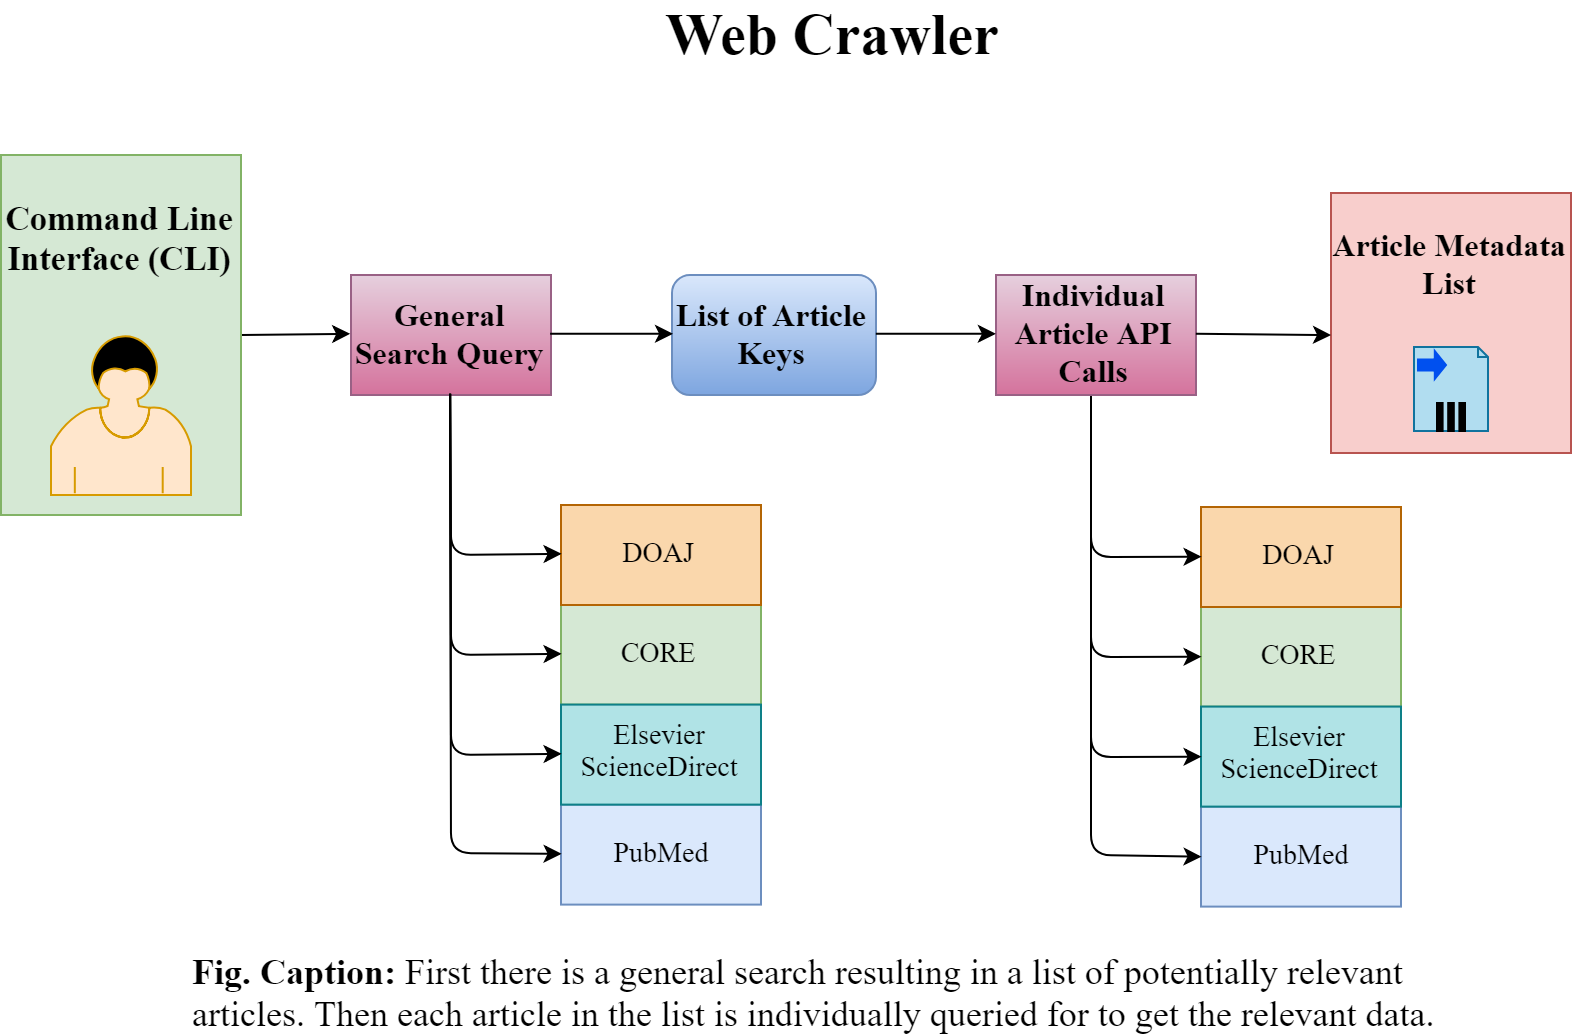
\includegraphics[scale=0.25]{Webcrawler_vJSHS1.0}
	\end{figure*}
	One of the main points of the web crawler is that it is federated and thus has the ability to dynamically allocate request loads out of the 4 databases. The reason why 4 databases are used instead of a singular database is because having 4 databases allows for more articles to be retrieved without surpassing API key load limitations along with opening up a wider breadth of articles to be retrieved. The REST API asynchronously sends the requests thus allowing for the web crawler to request articles without having to be bottlenecked by one particular database. In addition, the web crawler usually requests for extra article IDs from each database in order to ensure that there will be enough article IDs available in case of a rebalancing of each databases load. 
	After all of the articles are retrieved, they are packaged into a article list and then fed into the lexical-to-semantic converter to be converted to RDF triples. The citation metadata, however, is converted in this step using the Dublin Core ontology. It is only the textual aspects, the abstract and/or article text, that gets converted to RDF in the lexical-to-semantic converter.
	\subsection{Lexical-to-semantic converter}
	
	\quad The lexical-to-semantic converter is designed to translate the text of the article, which can either be just the abstract or the text of the paper itself, into semantic markup which describes the article. By converting the text of the article into linked data, it allows for the graphs of multiple articles to be merged. Thus the user can search the combined knowledge of multiple articles at once or specific aspects of a single article without actually having to read the article itself. The lexical-to-semantic converter consists of 3 steps: pre-processing, extraction, and conversion. Pre-processing deals with any tasks that depend upon the raw text of the article along with the creation of constituency trees based on the raw text. The extraction step primarily deals with the extraction of subject-verb-object triples from the constituency trees. Finally, in the post-processing step, the triples are converted to valid RDF and formatted into an RDF file. 
	\begin{figure*}[h!]
		\centering
		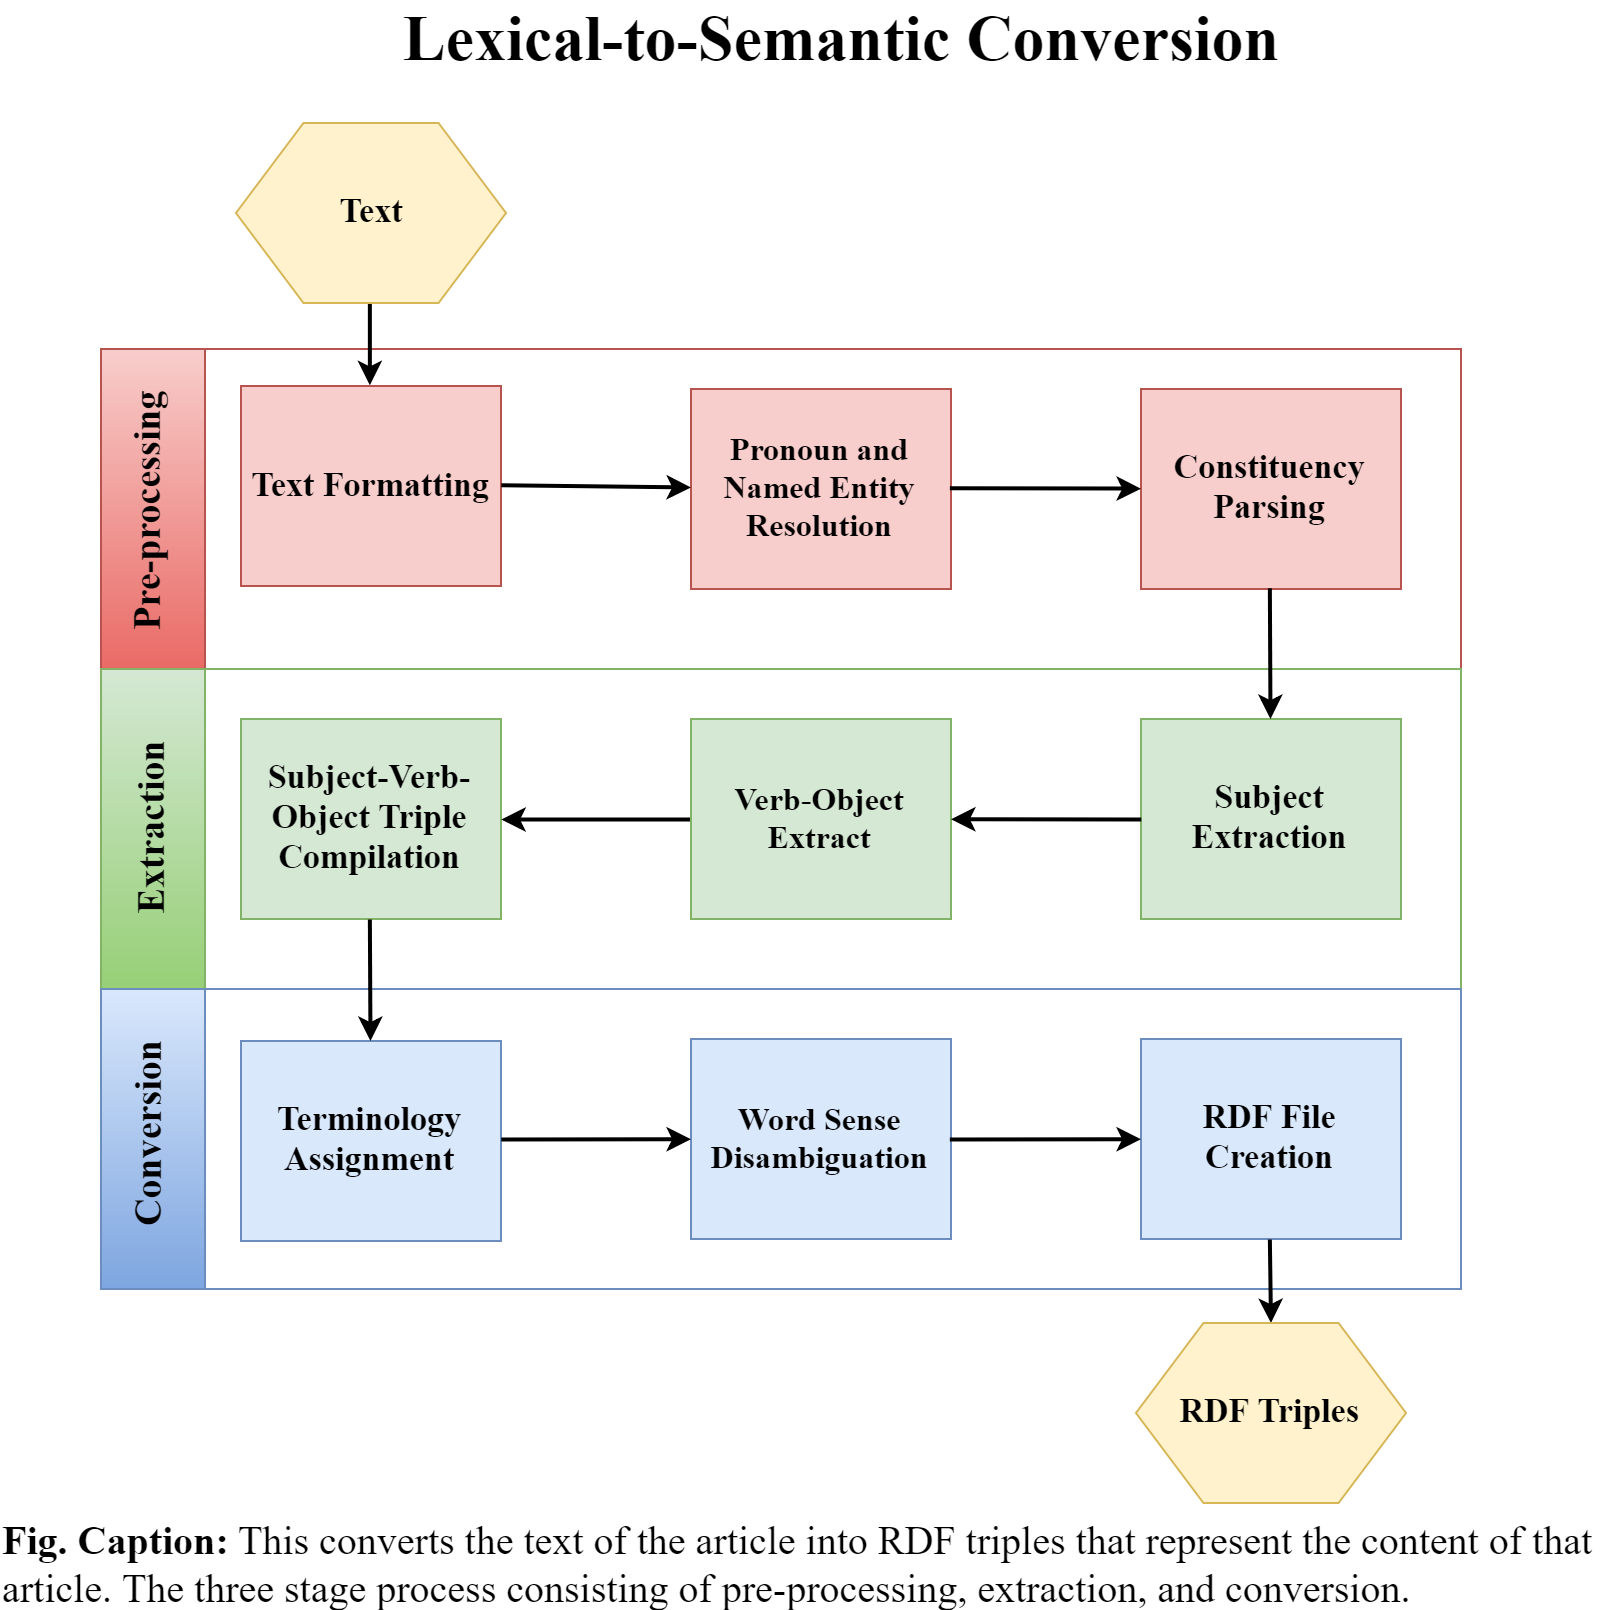
\includegraphics[scale=0.20]{NaturalLanguageProcessing_vJSHS2.0}
	\end{figure*}

	\subsubsection{Pre-processing} 
	\quad This step is designed to deal with steps that depend on the raw text of the document itself. First, the main body text is extracted from the file and any tags that are attached at the beginning or end are removed. The raw text is also re-spaced to correct for any variations in spacing formatting. Once the text is properly formatted, the nouns and pronouns are identified and cataloged. This is performed in a two step process. 
	The first is the use of pronoun resolution (also known as coreference resolution) to identify pronouns and their antecedents. The algorithm used for pronoun resolution is a statistical entity centric which allows for the use of contextual information. \cite{clark2015entity} The algorithm uses a trained classifier to prune mention pairs out of the initial search space. Then agglomerative clustering is used to merge the mention pair clusters together based on mention pair scores. This method allows for entity centric co-reference resolution which incorporates surrounding information.
	Once the pronouns are resolved, named entity recognition occurs. In this step any named entities are marked for later labeling in the conversion step. The Named Entity Recognition system works off of a supervised learning linear chain Conditional Random Field (CRF) sequence model \cite{finkel2005incorporating}. The model is able to discern long distance structures via the use of Gibbs sampling to enhance inferences in the probabilistic model. This allows for the accurate labeling of most named entities along with the ability to discern what type of entity that proper noun is, a feature that is useful for assigning URI’s to entities. 
	Paragraph formatting is then used to extract and separate paragraphs. This allows for the second step, which is the use of sentence parsing to separate sentences from one another. Though this may seem simple at first glance, there are various exceptions to deal with. For example, titles with the pattern of “Mr. Name” are similar to the pattern at the end of a sentence which is a period, space, then capital letter. To perform sentence parsing a classifier is trained to recognize various abbreviations, collocations, and words. 
	Once the sentence parsing occurs, a constituency parse is used in order to turn the sentence into a constituency tree. A constituency tree is a tree-based representation of the syntactic structure of a sentence in which the individual words are leaves and larger constructs of words (i.e. noun phrases, prepositional phrases, dependent clauses, etc.) are the nodes culminating in the source node representing the sentence. This works using a linear-time shift reduce constituency parser, which builds the constituency tree from the bottom-up using a series of transitions, each time correcting for grammar rules \cite{chen2014fast}. Utilizing a greedy approach, a neural network classifier predicts the correct transition based on features extracted from the sentence. This transition based approach is far faster than comparable algorithms due to the usage of a more dense feature set, which is beneficial for the already computationally intensive translator. 
	These are then converted to parented trees, trees in which each node/leaf has a reference to their parent, which allows for easier traversal along with the nodes having tags added to them to establish position and other lexical information for later use by the parser.
	
	\subsubsection{Extraction} 
	\quad In this step, the subject-verb-object triples are extracted from the constituency tree. First the independent clauses are split from each other by finding sub trees that are joined by conjunctions and qualify as independent clauses. This is done in order to allow for the noun and verb phrase searches to only have to deal with one general area at a time. Then breadth-first and depth-first search are used to find subject and verb-object phrases. The breadth-first search is used to find the highest noun phrase in the tree. This can be interpreted to be the main noun over the rest of the sentence. This noun phrase is then split up via conjunctions and any proximal adjectives are linked to the nouns. Then a two stage breadth-first, depth-first search is used to find the verb.
	%\begin{wrapfigure}{l}{0.5\linewidth}
	%	\centering
	%	%\rule{0.9\linewidth}{0.75\linewidth}
	%	\begin{center}
	%		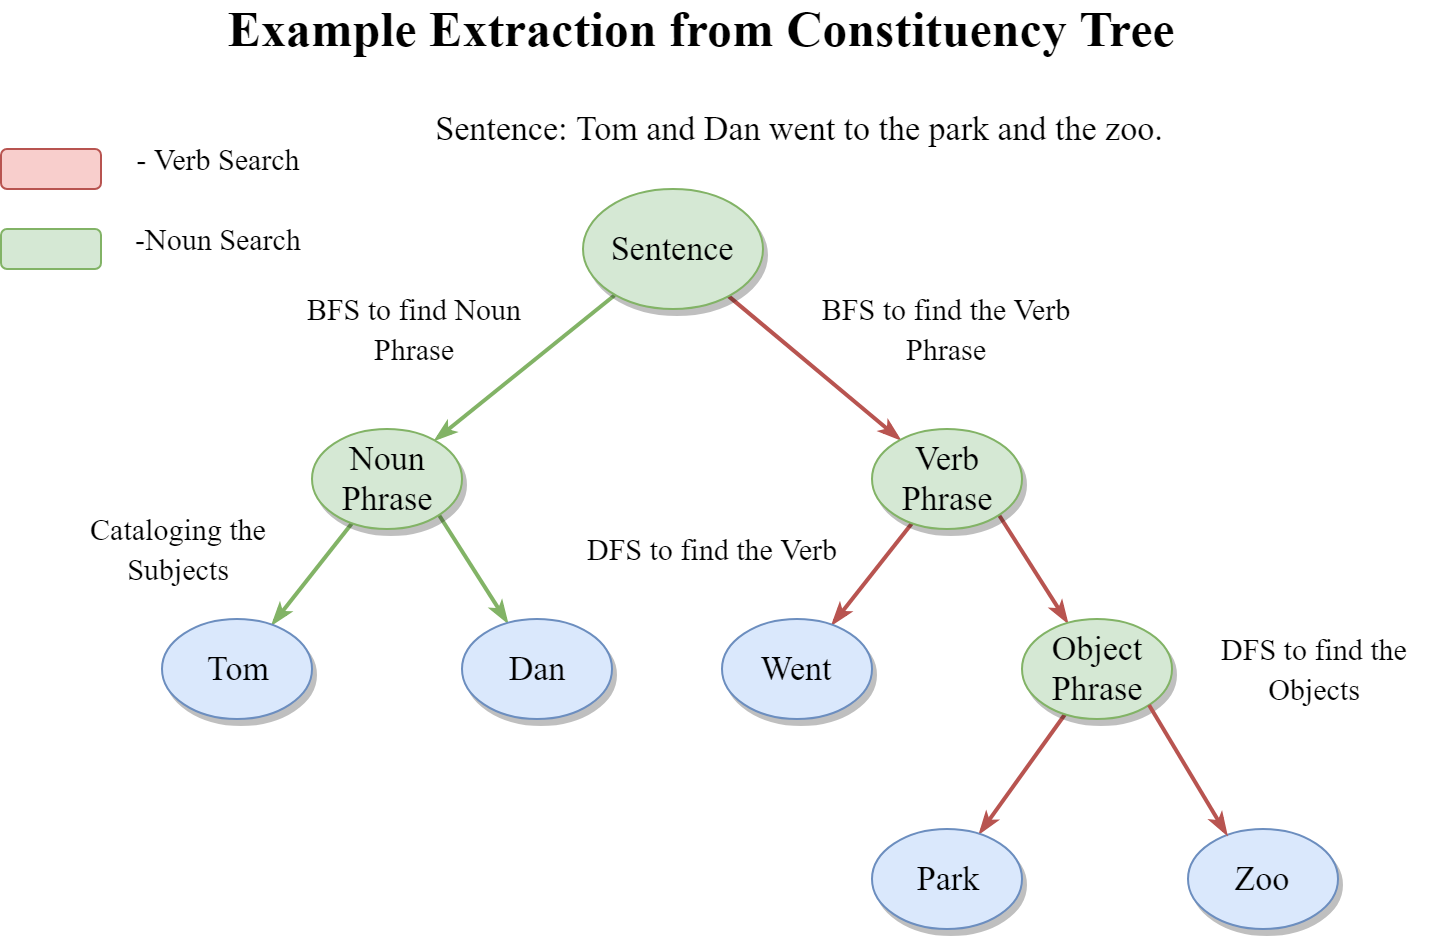
\includegraphics[scale=0.18]{ExampleExtraction_v2.0}
	%	\end{center}
	%\end{wrapfigure}
	Breadth first search is used to find the highest verb phrase. Then depth-first search is used to find the verb specifically so that it can be separated from the prepositional or adjective section of the verb phrase. The verb-object phrases are paired since, in general, the verb and object need to be specifically related by a link in order to maintain their relative positions. These phrases are then broken into their individual parts and tagged with positions. For the nouns, any proximal adjectives are put into a specialized adjectives list. This is so that they can be directly linked to their representative nouns. Then the noun and verb-object phrases are merged together to create subject-verb-object triples. These triples are able to roughly generalize a sentence’s contents. It should be noted that these differ from RDF triples due to the fact that RDF triples are encoded via URI’s, but currently these triples haven’t been properly encoded with URI’s, which brings us to our next step. 
	\subsubsection{Conversion} 
	\quad This step translates the logical form triples into RDF triples. It does this by assigning URI's to each part of the logical form triples. First "jargon" and some named entities are assigned URI's via databases such as MeSH \cite{lowe1994understanding}. Then word sense disambiguation is performed on standard words by assigning them to WordNet synsets, groupings of words that are semantically equivalent, using context and part of speech \cite{miller1995wordnet}. Word sense disambiguation allows the semantic markup to have non-specific references that represent the word’s meaning rather than its lexical form.  The algorithm that is used in order to perform this word sense disambiguation is Lesk \cite{banerjee2002adapted}. Lesk operates using a supervised classifier that compares the context that an ambiguous word is placed in to other example texts. This allows for the classifier to infer the semantic value of a word based on the context surrounding it.  Finally, named entities , numbers, dates, and other select non-standard parts of the triples are assigned to literals. One thing that should be noted is that the subject-verb-object triples aren’t directly translated to a single RDF triple. Rather the subject-verb-object triples are split into two triples: subject → performs → verb and verb → works on → object. This is due to two reasons. The first is that RDF triples can only use ontology based predicates, thus making it impossible for subject-verb-object triples to be directly translated to RDF triples without losing the semantic value of the verb. Thus the verb must be placed in a node so that its WordNet synset URI can be noted. The second reason is that the benefit of having the verb in a node is that it allows for more versatility on the user’s part since they can query the verb node via SPARQL for a variety of purposes. All of the translated RDF triples are then packaged into a named RDF graph.
	\begin{figure*}[h!]
		\centering
		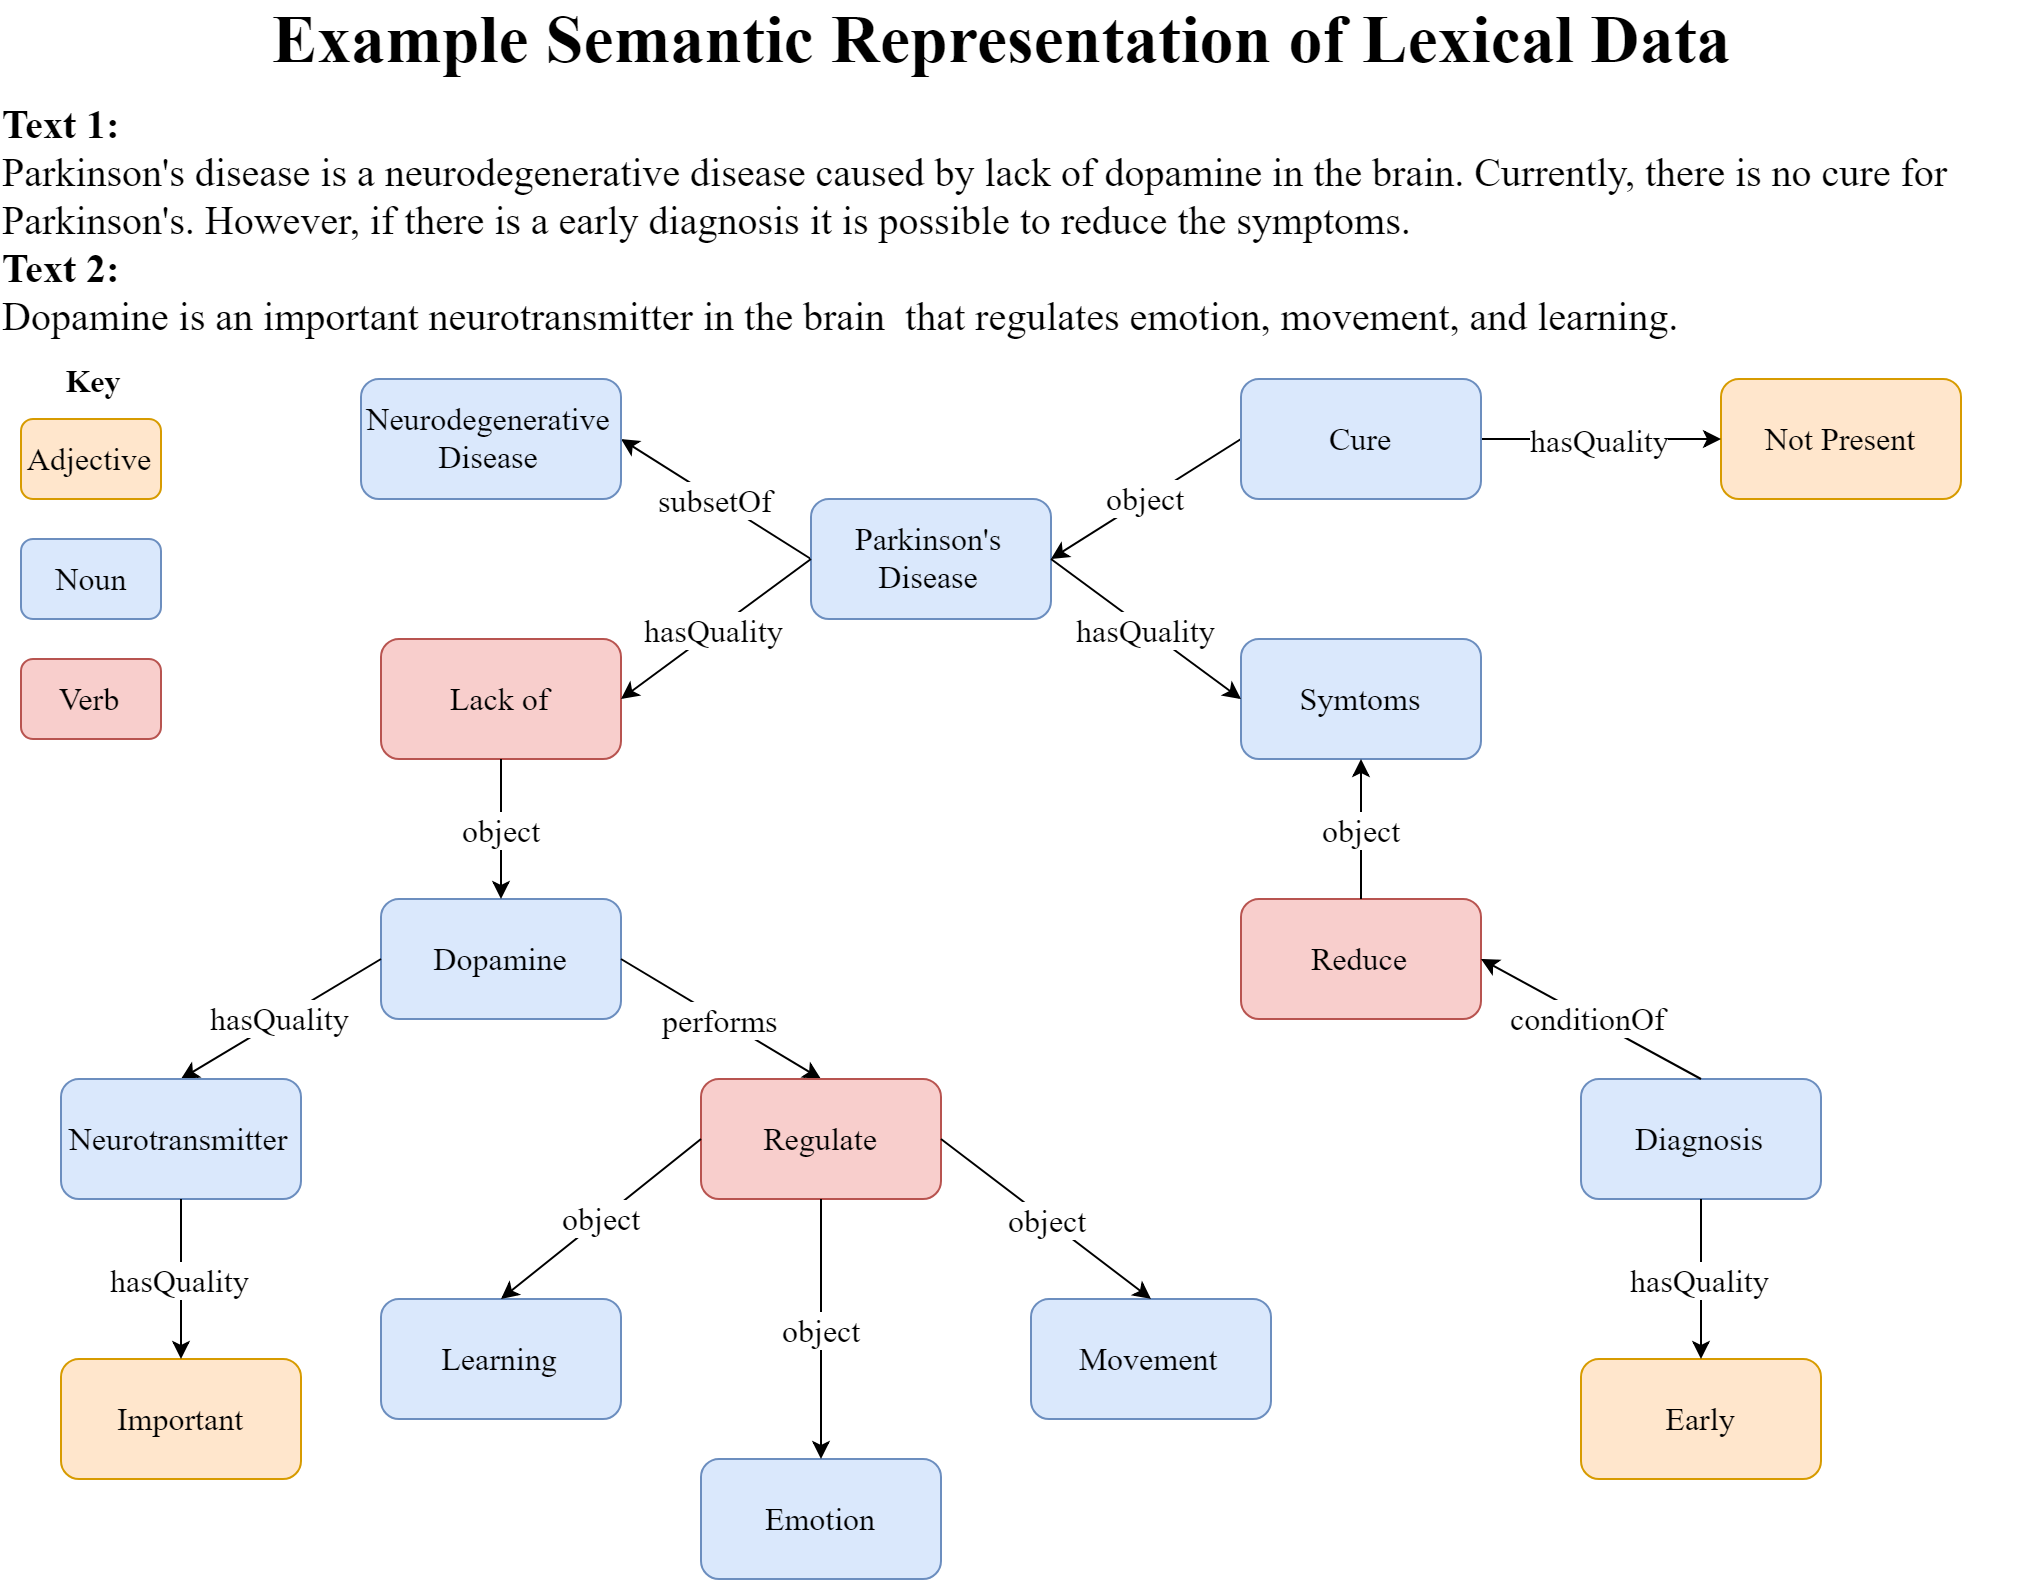
\includegraphics[scale=0.18]{ExampleRepresentation_vJSHS2.0}
	\end{figure*}
	
	\subsection{Triplestore}
	
	\quad Once the RDF graph is created, it is stored in the triplestore. Inside the triplestore is a set of RDF files, each of which describe an article. The triple store is primarily composed of flat text files which have XML formatted RDF graphs in them. XML is used since it is a far more universal encoding method than other encoding formats such as N3 or turtle. Even though there are alternatives that are more human-readable than the XML/RDF format, human readability should not be a concern given that only the decoder software will read the files. The XML format also allows it to be far more adaptable to storage in remote servers. In regards to the structure of each RDF file, the graph is split into two sections: the citation metadata section and the text representation section. The citation metadata section holds information about the articles such as title, author name, publication date, etc. This is represented using the Dublin Core ontology \cite{weibel1998dublin}. 
	The text representation section hold the triples that have been extracted by the lexical-to-semantic converter. These triples are a graph-based description of the text of the article (which can be the actual article and/or the abstract). The triple store has two possible locations to be stored on. It can be stored online on a server via REST API and it can also be stored locally on the computer. By storing the records on the server, the searches of individual users can help to augment the search results of other users, allowing for the gradual construction of a linked data representation of all articles. 
	
	\subsection{Internal Search Engine}
	
	\subsubsection{SPARQL Search}
	\quad The internal search engine is used to search through all of the converted articles for information that the user has requested. The internal search engine is based on the SPARQL Protocol and RDF Query Language (SPARQL), the W3C standard query language for RDF. SPARQL operates by having a series of conditions which are inputted by the user to narrow down values of interest which can be returned. SPARQL loops through all of the triples (which are effectively edges) in a given graph and filters them based on user inputted conditions. Since these condition can be linked together, the results from one condition can be entered into the next. What this allows a user to do is effectively to traverse the graph searching for answers to a question. Using the SPARQL conditions, the user can specify a part of the graph (subgraph) that they want to retrieve. Then they can further specify which parts of the subgraph they want returned to them. The conditions come in the form of triples with some parts being variables, allowing any value to be stored there. Other values are set, thus meaning that for a triple to pass the filter it must have a matching value at that position. The user then inputs which variables they want returned to them. SPARQL syntax has many other operations available such as having optional conditions, including sub-queries, and manipulating the values of variables. The versatility of SPARQL makes it an ideal basis for the search engine. 
	Search Engine: The search engine operates by constructing a singular local graph on the machine that is performing the query. Though this is certainly very memory intensive for the host machine, it allows for the search engine to be extremely versatile with the queries it performs. If the search engine was federated, then the search engine could only search inside articles themselves. When the local graph is created, the SPARQL query is run on the unified graph and the results are sent to the user along with the provenance article of each result, in case the user wishes to look more into the article of origin for a particular result. The SPARQL Query can either be inputted directly by a user or it can be built via the query builder. The results of the query are in a list format with each row representing a resultant subgraph and each column representing a section of each subgraph.
	\begin{figure*}[h!]
		\centering
		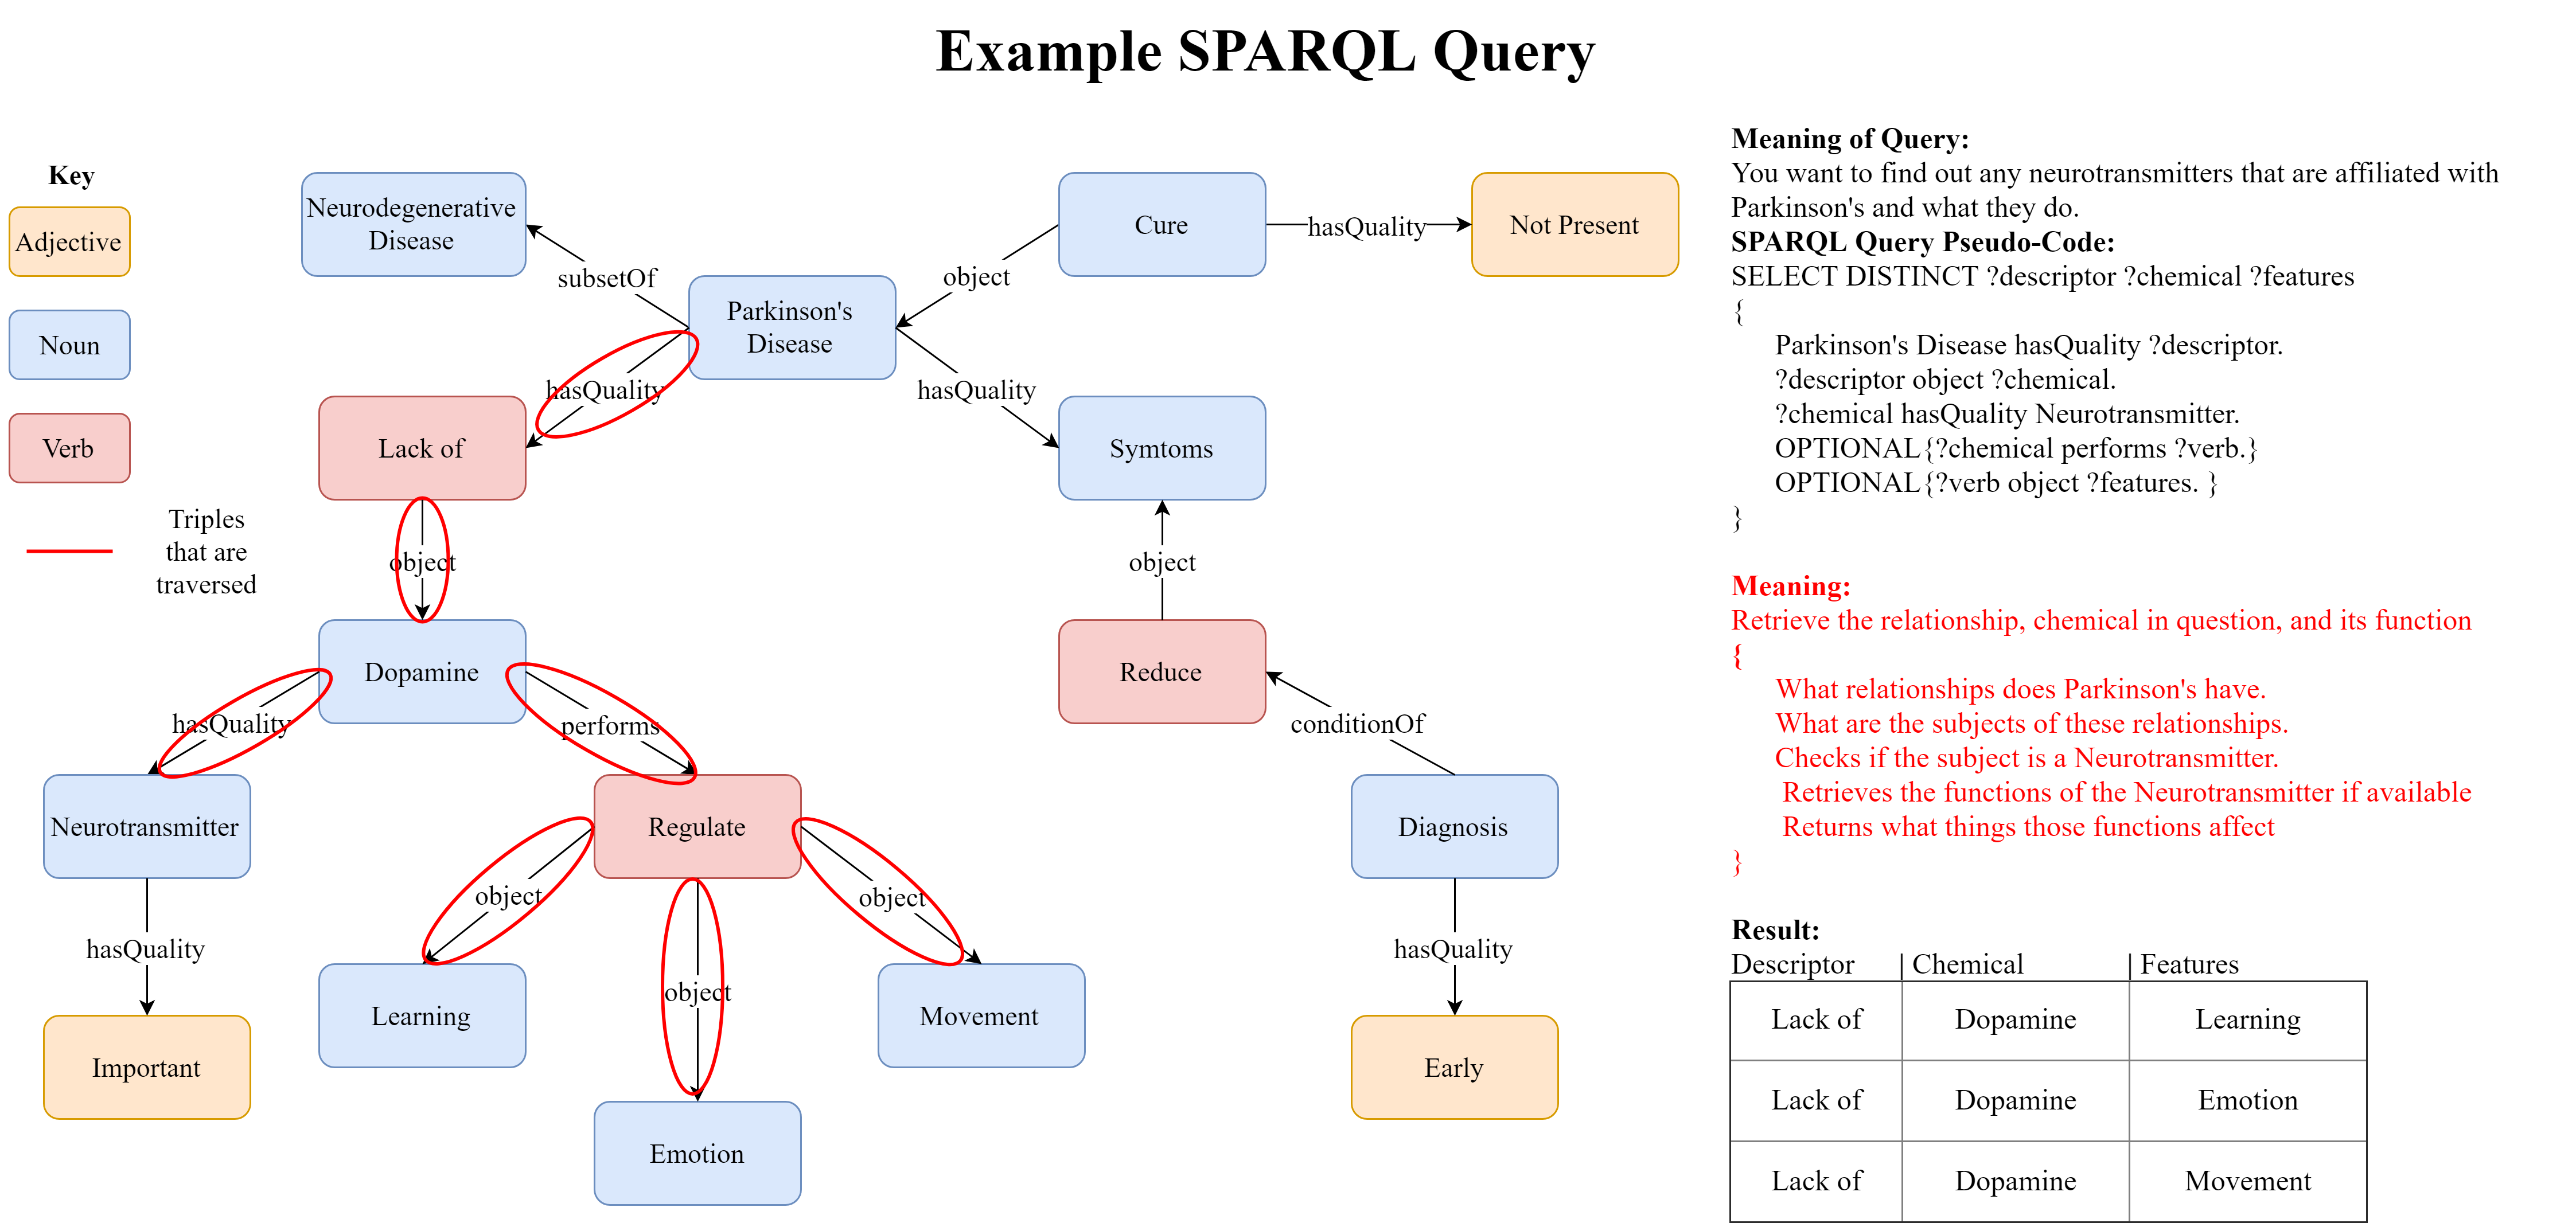
\includegraphics[scale=0.11]{ExampleSPARQL_vJSHS2.0}
	\end{figure*}
	\subsubsection{Query Builder}
	\quad One of the primary drawbacks of SPARQL is that in spite of its versatility, it is a query language. Thus, for an average user, it is extremely difficult to learn SPARQL due to its complexity. In order to solve this, a SPARQL builder form was designed that is capable of building SPARQL queries for the user. The SPARQL builder is primarily designed to work exclusively for SELECT type SPARQL queries which means that it is optimized to retrieve answers for a user. The other types of queries are the CONSTRUCT, ASK, and DESCRIBE queries. Though these are supported by the search engine, they cannot be built via the query builder and thus must be inputted directly by the user. 
	\begin{figure*}[h!]
		\centering
		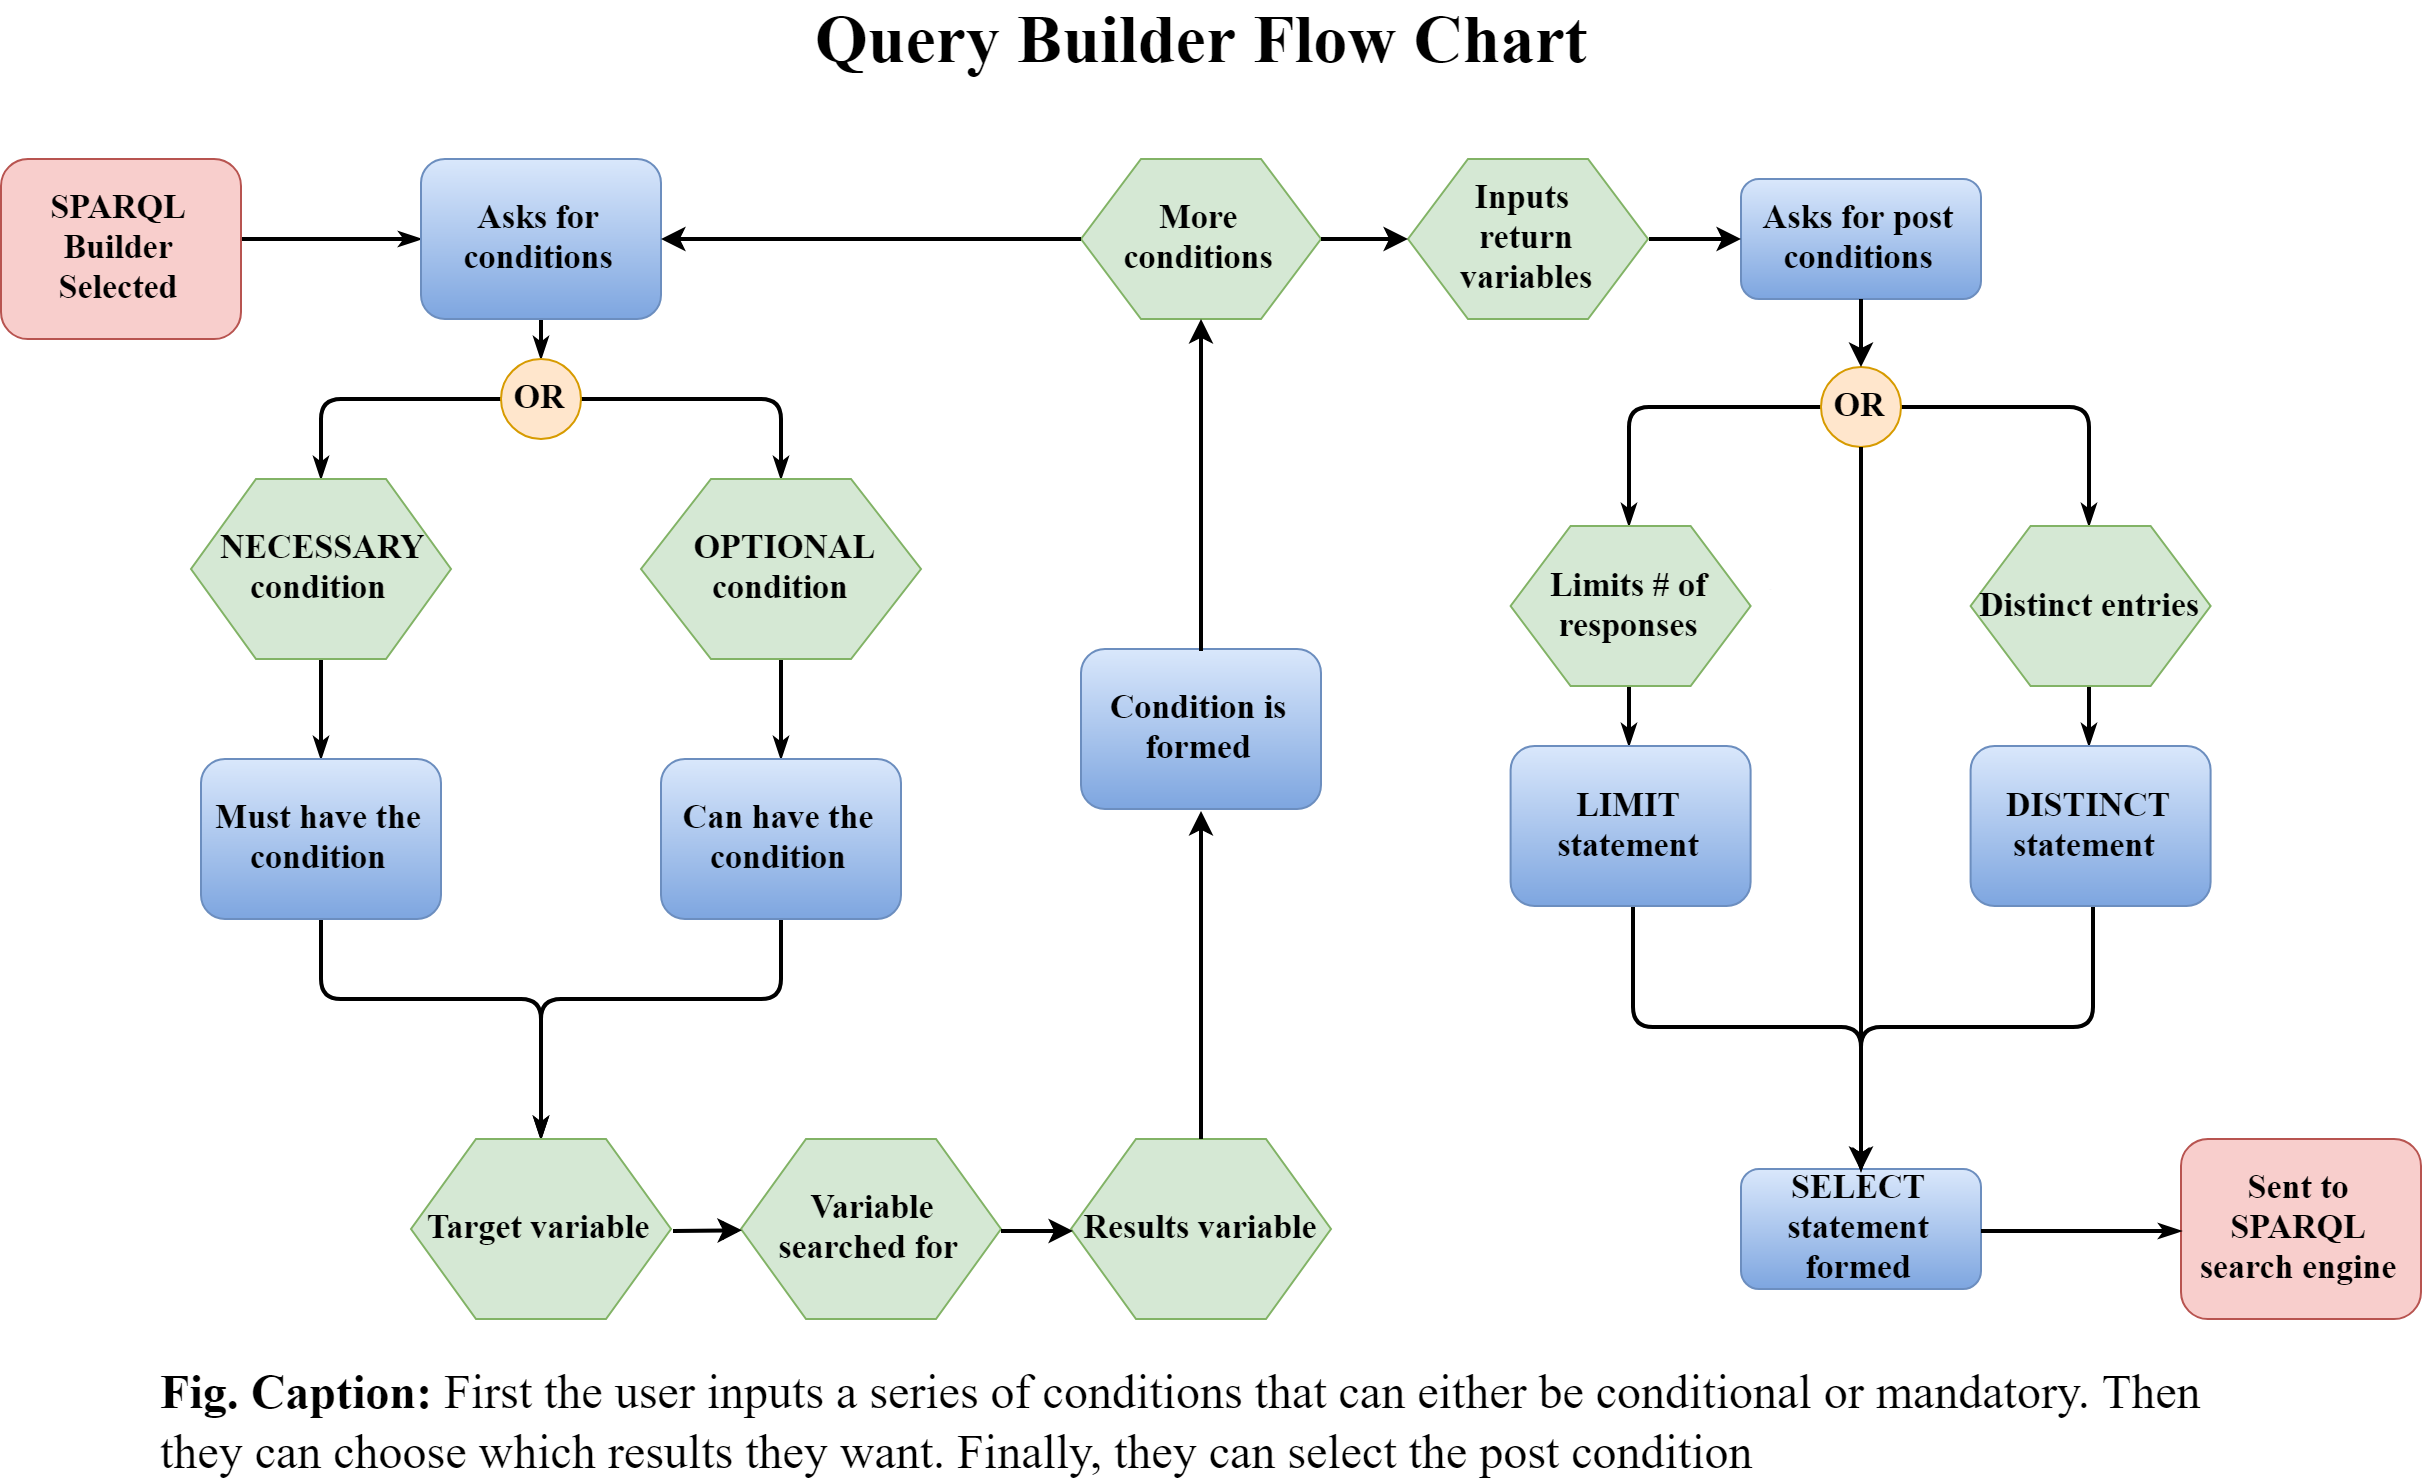
\includegraphics[scale=0.17]{Builderform_vJSHS2.0}
	\end{figure*}
	\quad The Query Builder operates in a series of steps. First the user is asked to input a set of conditions, each with 4 parts. The first part indicates whether or not the condition is mandatory, the second indicates the target variable, the third indicates the target action and the 4th indicates the result variable. It should be noted that the last 3 parts correspond to the 3 parts of an RDF triple. This is because these conditions act as filters for triples in which triples can only be accepted if they pass the condition. The result of one condition can be used as the subject for the next, allowing users to make a set of triples which is used to specify a particular area of the graph. Once the user is done inputting triples, the user can choose which variables they want to get returned to them along with setting post-conditions. An example of a post-condition is setting a limit on the number of articles that are returned. Though this builder form doesn’t perfectly replicate the capabilities of SPARQL syntax, for example losing some functionality with variable value manipulation, it is a potent resource for users who don’t know SPARQL. 
	\section{Results}
	\subsection{General Computational Performance}
	\quad All of these tests where performed on a computer running on Windows 10 Pro. The computer has an Intel i7-8750HK Hexa-core CPU clocked to 3.7GHz, 16Gb of DDR4 RAM, and a Nvidia GTX 1070 Graphics Card with 8Gb of VRAM. The network that this was run on has a 30.3 Mbps download and 5.94 Mbps upload speed. The process was single-threaded and didn't make use of any form of GPU acceleration. 
	
	For the tests, the number of triples in the triple store initially is none. The only triples that are present are the ones being added by the query. For results, a result indicates a particular set of triples that satisfies the SPARQL search condition and the number of triples indicates the number of specified variables that were returned to the user. In this instance, there were two specified variables: author and title.
	
	\scalebox{0.71}{%
		\centering
		\begin{tabular}{|l|l|l|l|l|l|l|}
			\hline
			\multicolumn{3}{|l|}{\textbf{Input}}                                                                                                                                                                                                                                                                                                                                                                                                                & \multicolumn{2}{l|}{\textbf{Details}}                                                                                                                                & \multicolumn{2}{l|}{\textbf{Performance}}                                                                                       \\ \hline
			\begin{tabular}[c]{@{}l@{}}General Search \\ Query\end{tabular}                                                    & \begin{tabular}[c]{@{}l@{}}Number of \\ Articles \\ Requested\end{tabular} & Semantic Search Query                                                                                                                                                                                                                             & \begin{tabular}[c]{@{}l@{}}Number of \\ Articles \\ Retrieved\end{tabular} & \begin{tabular}[c]{@{}l@{}}Number of \\ Abstracts and \\ Triples Converted\end{tabular} & Results                                                            & Runtime                                                    \\ \hline
			\multirow{3}{*}{\textbf{Fluid Dynamics}}                                                                           & \textit{10 articles}                                                       & \multirow{6}{*}{\begin{tabular}[c]{@{}l@{}}Meaning:\\ Asking for the title and author \\ of each article\\ Query:\\ SELECT DISTINCT ?author ?title\\ WHERE \{\\       ?a dc:contributor ?author .\\       ?a dc:title ?title .\\ \}\end{tabular}} & 10 articles                                                                & \begin{tabular}[c]{@{}l@{}}10 abstracts\\ 369 triples\end{tabular}                      & \begin{tabular}[c]{@{}l@{}}10 results\\ 20 triples\end{tabular}    & \begin{tabular}[c]{@{}l@{}}37.12 \\ seconds\end{tabular}   \\ \cline{2-2} \cline{4-7} 
			& \textit{100 articles}                                                      &                                                                                                                                                                                                                                                   & 100 articles                                                               & \begin{tabular}[c]{@{}l@{}}98 abstracts\\ 3834 triples\end{tabular}                     & \begin{tabular}[c]{@{}l@{}}98 results\\ 196 triples\end{tabular}   & \begin{tabular}[c]{@{}l@{}}312.34 \\ seconds\end{tabular}  \\ \cline{2-2} \cline{4-7} 
			& \textit{1000 articles}                                                     &                                                                                                                                                                                                                                                   & 997 articles                                                               & \begin{tabular}[c]{@{}l@{}}956 abstracts\\ 27428 triples\end{tabular}                   & \begin{tabular}[c]{@{}l@{}}956 results\\ 1912 triples\end{tabular} & \begin{tabular}[c]{@{}l@{}}2589.32 \\ seconds\end{tabular} \\ \cline{1-2} \cline{4-7} 
			\multirow{3}{*}{\textbf{\begin{tabular}[c]{@{}l@{}}MRI Scans of \\ Neuro-\\ degenerative\\ Diseases\end{tabular}}} & \textit{10 articles}                                                       &                                                                                                                                                                                                                                                   & 10 articles                                                                & \begin{tabular}[c]{@{}l@{}}10 abstracts\\ 293 triples\end{tabular}                      & \begin{tabular}[c]{@{}l@{}}10 results\\ 20 triples\end{tabular}    & \begin{tabular}[c]{@{}l@{}}31.84 \\ seconds\end{tabular}   \\ \cline{2-2} \cline{4-7} 
			& \textit{100 articles}                                                      &                                                                                                                                                                                                                                                   & 100 articles                                                               & \begin{tabular}[c]{@{}l@{}}100 abstracts\\ 3223 triples\end{tabular}                    & \begin{tabular}[c]{@{}l@{}}100 results\\ 200 triples\end{tabular}  & \begin{tabular}[c]{@{}l@{}}283.31 \\ seconds\end{tabular}  \\ \cline{2-2} \cline{4-7} 
			& \textit{1000 articles}                                                     &                                                                                                                                                                                                                                                   & 994 articles                                                               & \begin{tabular}[c]{@{}l@{}}973 abstracts\\ 31568 triples\end{tabular}                   & \begin{tabular}[c]{@{}l@{}}973 results\\ 1946 triples\end{tabular} & \begin{tabular}[c]{@{}l@{}}2391.12 \\ seconds\end{tabular} \\ \hline
		\end{tabular}
	}
	
	Unless otherwise stated, only the abstracts had triples extracted from them, and not whole articles. This is because the the number of articles that have their full text available is limited, and thus would impact the results of the tests irregularly. Thus, to simplify the results, only triples coming from abstracts have been extracted, thus eliminating the uncontrolled variable of whether or not a particular article has full text available.
	\subsection{Individual Performance Breakdown Per Section}
	\subsubsection{Web Crawler}
	The web crawler tests focused on the individualized retrieval performance for each of the 4 databases that SHIRASE accesses: DOAJ, Elsevier ScienceDirect, PubMed, and CORE. For each of these, a general search query was inputted along with a specified amount of articles requested. Then the table shows the number of articles that they managed to retrieve along with the runtime.
	
	\scalebox{0.8}{
		\centering
		\begin{tabular}{|l|l|l|l|l|}
			\hline
			\begin{tabular}[c]{@{}l@{}}Target \\ Database\end{tabular}                                  & General Search Query                                                                               & \begin{tabular}[c]{@{}l@{}}Number of Articles\\ Requested\end{tabular} & \begin{tabular}[c]{@{}l@{}}Number of Articles \\ Returned\end{tabular} & Runtime                                                   \\ \hline
			\multirow{3}{*}{\textbf{DOAJ}}                                                              & \multirow{3}{*}{\textit{\begin{tabular}[c]{@{}l@{}}Dementia \\ Symptoms\end{tabular}}}             & 10 Articles                                                            & 10 articles                                                            & \begin{tabular}[c]{@{}l@{}}15.13 \\ seconds\end{tabular}  \\ \cline{3-5} 
			&                                                                                                    & 100 Articles                                                           & 100 articles                                                           & \begin{tabular}[c]{@{}l@{}}93.46 \\ seconds\end{tabular}  \\ \cline{3-5} 
			&                                                                                                    & 1000 Articles                                                          & 983 articles                                                           & \begin{tabular}[c]{@{}l@{}}836.17 \\ seconds\end{tabular} \\ \hline
			\multirow{3}{*}{\textbf{\begin{tabular}[c]{@{}l@{}}Elsevier \\ ScienceDirect\end{tabular}}} & \multirow{3}{*}{\textit{\begin{tabular}[c]{@{}l@{}}Semantic \\ Knowledge \\ Graphs\end{tabular}}}  & 10 Articles                                                            & 10 articles                                                            & \begin{tabular}[c]{@{}l@{}}17.32 \\ seconds\end{tabular}  \\ \cline{3-5} 
			&                                                                                                    & 100 Articles                                                           & 100 articles                                                           & \begin{tabular}[c]{@{}l@{}}104.32 \\ seconds\end{tabular} \\ \cline{3-5} 
			&                                                                                                    & 1000 Articles                                                          & 998 articles                                                           & \begin{tabular}[c]{@{}l@{}}934.74 \\ seconds\end{tabular} \\ \hline
			\multirow{3}{*}{\textbf{PubMed}}                                                            & \multirow{3}{*}{\textit{MRI Breast Cancer}}                                                        & 10 Articles                                                            & 10 articles                                                            & \begin{tabular}[c]{@{}l@{}}13.33 \\ seconds\end{tabular}  \\ \cline{3-5} 
			&                                                                                                    & 100 Articles                                                           & 100 articles                                                           & \begin{tabular}[c]{@{}l@{}}91.45 \\ seconds\end{tabular}  \\ \cline{3-5} 
			&                                                                                                    & 1000 Articles                                                          & 1000 articles                                                          & \begin{tabular}[c]{@{}l@{}}794.95 \\ seconds\end{tabular} \\ \hline
			\multirow{3}{*}{\textbf{CORE}}                                                              & \multirow{3}{*}{\textit{\begin{tabular}[c]{@{}l@{}}Convolutional \\ Neural Networks\end{tabular}}} & 10 Articles                                                            & 10 articles                                                            & \begin{tabular}[c]{@{}l@{}}20.42 \\ seconds\end{tabular}  \\ \cline{3-5} 
			&                                                                                                    & 100 Articles                                                           & 99 articles                                                            & \begin{tabular}[c]{@{}l@{}}118.96 \\ seconds\end{tabular} \\ \cline{3-5} 
			&                                                                                                    & 1000 Articles                                                          & 973 articles                                                           & \begin{tabular}[c]{@{}l@{}}989.49 \\ seconds\end{tabular} \\ \hline
		\end{tabular}
	}
	\subsubsection{Lexical to Semantic Translation}
	The lexical to semantic translation table shows the amount of triples extracted from a set amount of articles. The number of words column indicates the total number of words and average number of words per article. The first section is just the abstracts being converted. The second section is the full-text of the article being converted. It should be noted that the articles being converted in the first section are not the same as the articles being converted in the second section.
	
	\scalebox{0.8}{
		\begin{tabular}{|l|l|l|l|l|}
			\hline
			Translation                & Number of Articles & \# of Words                                                                          & \begin{tabular}[c]{@{}l@{}}\# of Abstract Triples \\ Extracted\end{tabular}            & Runtime                                                   \\ \hline
			\multirow{3}{*}{Abstract}  & 10 articles        & \begin{tabular}[c]{@{}l@{}}Total: 2131 words\\ Average: 213.1 words\end{tabular}     & \begin{tabular}[c]{@{}l@{}}Total: 327 triples\\ Average: 32.7 triples\end{tabular}     & \begin{tabular}[c]{@{}l@{}}20.23\\ seconds\end{tabular}   \\ \cline{2-5} 
			& 100 articles       & \begin{tabular}[c]{@{}l@{}}Total: 22423 words\\ Average: 224.23 words\end{tabular}   & \begin{tabular}[c]{@{}l@{}}Total: 2789 triples\\ Average: 27.89 triples\end{tabular}   & \begin{tabular}[c]{@{}l@{}}211.23\\ seconds\end{tabular}  \\ \cline{2-5} 
			& 1000 articles      & \begin{tabular}[c]{@{}l@{}}Total: 253123 words\\ Average: 253.123 words\end{tabular} & \begin{tabular}[c]{@{}l@{}}Total: 29854 triples\\ Average: 29.85 triples\end{tabular}  & \begin{tabular}[c]{@{}l@{}}1814.69\\ seconds\end{tabular} \\ \hline
			\multirow{3}{*}{Full-Text} & 5 articles         & \begin{tabular}[c]{@{}l@{}}Total: 20615 words\\ Average: 4123 words\end{tabular}     & \begin{tabular}[c]{@{}l@{}}Total: 3173 triples\\ Average: 634.6 triples\end{tabular}   & \begin{tabular}[c]{@{}l@{}}305.67\\ seconds\end{tabular}  \\ \cline{2-5} 
			& 10 articles        & \begin{tabular}[c]{@{}l@{}}Total: 51261 words\\ Average: 5126.1 words\end{tabular}   & \begin{tabular}[c]{@{}l@{}}Total: 7123 triples\\ Average: 712.3 triples\end{tabular}   & \begin{tabular}[c]{@{}l@{}}575.64\\ seconds\end{tabular}  \\ \cline{2-5} 
			& 20 articles        & \begin{tabular}[c]{@{}l@{}}Total: 97526 words\\ Average: 4876 words\end{tabular}     & \begin{tabular}[c]{@{}l@{}}Total: 13783 triples\\ Average: 689.15 triples\end{tabular} & \begin{tabular}[c]{@{}l@{}}1125.43\\ seconds\end{tabular} \\ \hline
		\end{tabular}
	}
	\subsubsection{Internal Search}
 
	
	\scalebox{0.67}{
		\begin{tabular}{|l|l|l|l|l|}
			\hline
			Size of Triplestore                                                                                   & SPARQL Search Query                                                                                                                                                                                                                                                                                                                                                                                                                                                                      & Meaning                                                                                                                                                              & Result                                                              & Runtime                                                   \\ \hline
			\multirow{2}{*}{\textbf{\begin{tabular}[c]{@{}l@{}}$\sim$1000 triples\\ 65 articles\end{tabular}}}    & \begin{tabular}[c]{@{}l@{}}SELECT DISTINCT ?author ?title\\ WHERE \{\\       ?a dc:contributor ?author .\\       ?a dc:title ?title .\\ \}\end{tabular}                                                                                                                                                                                                                                                                                                                                  & \begin{tabular}[c]{@{}l@{}}Requesting for the \\ author of the article \\ and the title.\end{tabular}                                                                & \begin{tabular}[c]{@{}l@{}}130 results\\ 260 triples\end{tabular}   & \begin{tabular}[c]{@{}l@{}}4.32 \\ seconds\end{tabular}   \\ \cline{2-5} 
			& \begin{tabular}[c]{@{}l@{}}@prefix xsd: \textless{}http://www.w3.org/2001/XMLSchema\#\textgreater .\\ SELECT DISTINCT ?database ?title\\ \{\\       ?article dc:created ?date\\        FILTER(?date \textgreater "2014-05-23T10:20:13+05:30"\\        \textasciicircum{}\textasciicircum{}xsd:dateTime)\\        ?article dc:publisher ?database\\        FILTER(?database = "PubMed"\textasciicircum{}\textasciicircum{}xsd:string\\        ?article dc:title ?title\\ \}\end{tabular}  & \begin{tabular}[c]{@{}l@{}}Requesting for articles \\ that have been published\\ after May 23, 2014 and\\ come specifically from\\ the PubMed database.\end{tabular} & \begin{tabular}[c]{@{}l@{}}12 articles\\ 24 triples\end{tabular}    & \begin{tabular}[c]{@{}l@{}}5.12 \\ seconds\end{tabular}   \\ \hline
			\multirow{2}{*}{\textbf{\begin{tabular}[c]{@{}l@{}}$\sim$10000 triples\\ 578 articles\end{tabular}}}  & \begin{tabular}[c]{@{}l@{}}SELECT DISTINCT ?author ?title\\ WHERE \{\\       ?a dc:contributor ?author .\\       ?a dc:title ?title .\\ \}\end{tabular}                                                                                                                                                                                                                                                                                                                                  & \begin{tabular}[c]{@{}l@{}}Requesting for the \\ author of the article and\\ the title.\end{tabular}                                                                 & \begin{tabular}[c]{@{}l@{}}578 results\\ 1156 triples\end{tabular}  & \begin{tabular}[c]{@{}l@{}}41.11 \\ seconds\end{tabular}  \\ \cline{2-5} 
			& \begin{tabular}[c]{@{}l@{}}@prefix xsd: \textless{}http://www.w3.org/2001/XMLSchema\#\textgreater .\\ SELECT DISTINCT ?database ?author\\ \{\\       ?article dc:created ?date\\        FILTER(?date \textgreater "2014-05-23T10:20:13+05:30"\\        \textasciicircum{}\textasciicircum{}xsd:dateTime)\\        ?article dc:publisher ?database\\        FILTER(?database = "PubMed"\textasciicircum{}\textasciicircum{}xsd:string\\        ?article dc:title ?title\\ \}\end{tabular} & \begin{tabular}[c]{@{}l@{}}Requesting for articles \\ that have been published\\ after May 23, 2014 and\\ come specifically from\\ the PubMed database.\end{tabular} & \begin{tabular}[c]{@{}l@{}}132 results\\ 264 triples\end{tabular}   & \begin{tabular}[c]{@{}l@{}}45.32 \\ seconds\end{tabular}  \\ \hline
			\multirow{2}{*}{\textbf{\begin{tabular}[c]{@{}l@{}}$\sim$30000 triples\\ 1673 articles\end{tabular}}} & \begin{tabular}[c]{@{}l@{}}SELECT DISTINCT ?author ?title\\ WHERE \{\\       ?a dc:contributor ?author .\\       ?a dc:title ?title .\\ \}\end{tabular}                                                                                                                                                                                                                                                                                                                                  & \begin{tabular}[c]{@{}l@{}}Requesting for the \\ author of the article and\\ the title.\end{tabular}                                                                 & \begin{tabular}[c]{@{}l@{}}1673 results\\ 3346 triples\end{tabular} & \begin{tabular}[c]{@{}l@{}}127.21 \\ seconds\end{tabular} \\ \cline{2-5} 
			& \begin{tabular}[c]{@{}l@{}}@prefix xsd: \textless{}http://www.w3.org/2001/XMLSchema\#\textgreater .\\ SELECT DISTINCT ?database ?author\\ \{\\       ?article dc:created ?date\\        FILTER(?date \textgreater "2014-05-23T10:20:13+05:30"\\        \textasciicircum{}\textasciicircum{}xsd:dateTime)\\        ?article dc:publisher ?database\\        FILTER(?database = "PubMed"\textasciicircum{}\textasciicircum{}xsd:string\\        ?article dc:title ?title\\ \}\end{tabular} & \begin{tabular}[c]{@{}l@{}}Requesting for articles \\ that have been published\\ after May 23, 2014 and\\ come specifically from\\ the PubMed database.\end{tabular} & \begin{tabular}[c]{@{}l@{}}346 results\\ 692 triples\end{tabular}   & \begin{tabular}[c]{@{}l@{}}134.87 \\ seconds\end{tabular} \\ \hline
		\end{tabular}
	}

	For the internal search, there is a set number of triples present in the triple store for each internal search. Two internal searches have been run: one regarding basic citation metadata and another regarding specific information.
	\section{Discussion}
	\subsection{Discussion of the Computational Performance}
    \quad The results of SHIRASE are relatively promising. For the general test of computational performance the runtime seemed to scale more or less linearly to the amount of articles requested. However, there seems to be a constant time process, most likely stemming from the time required for the initial search of the databases with the general search query. Both the time to retrieve the individual article metadata and the time to extract the triples from the abstract seem to scale linearly, with some minor variability. The system takes less than a minute for 10 articles, 5 minutes for a 100 articles, and 40 minutes for a 1000 articles. Another point of interest to note is that the number of abstracts converted is less than the number of articles retrieved. This is because the system cannot parse the abstract due to particularly advanced sentence structure or other features that cannot be recognized.  
    
    This conclusion that most of the runtime is taken up by the retrieval and conversion phases is lended credence to by the results from the web crawler performance tests. They show that retrieving the articles from the databases takes up nearly a third of the runtime of the search. The results of the tests are split by database. Analysis indicates that some databases have faster response times than others. For example, PubMed seems to be the fastest while CORE is the slowest. However, these response differences seem to be relatively minor. A more major point is that as the number of requested articles increases, the number of articles being dropped by the web crawler also increases. The web crawler rejecting an article can occur due to a few reasons. The most notable reason is that some articles may be written in languages other than English, thus requiring them to be rejected by the web crawler as the lexical-to-semantic translator doesn't support other languages.
    
    Although the web crawler takes up a significant amount of runtime, the step that takes up the most amount of time is the lexical to semantic translation. In general, the lexical to semantic translation seems to take up approximately 2/3 of the complete search runtime. It also appears that the runtime scaling is linear with the size of the articles. Of course, there is a large amount of variability on a case to case basis due to differing sentence structures, required noun processing, and differences in content that has to parsed into RDF. However, these variances average out to form a roughly linear relation between runtime and length. 
   
    The runtime complexity of the SPARQL Search Query is extremely fast compared to the runtimes of the retrieval and translation steps, taking an extremely small time of the process. In fact, it seems that the runtimes for the simple query and the more complex SPARQL query are nearly identical. This may indicate that the runtime for the internal search is independent of query complexity, which is better for advanced searches. However, compared to its conventional contemporaries, the internal search seems extremely slow. The internal search's time complexity scales linearly with the size of the triplestore. This makes it so that a search of 30000 triples takes nearly 2 minutes to complete. This is problematic since a complete semantic graph would hypothetically consist of millions or billions of triples. The reason for this high time complexity is due to the method of the search. Currently, the system compiles all of the RDF files in a merged local graph. This graph is then searched through by the search engine. Because it relies on merging all of the resources on the triplestore to perform a search, it takes approximately linear time complexity to search the graph. Hopefully, this can be remedied by further improvements to the internal search engine.
	\subsection{Possible Expansions}
	\subsubsection{General Expansion}
	\quad The most obvious direction for expansion is to generalize the system. Currently, SHIRASE is specialized for researchers and is limited to article search functionality. The next logical step would be to generalize the system to a wide variety of content types including chat boards, social media, video streaming sites, and blogs. The largest change would be to lexical to semantic parsing. For example, far less formal grammar is used on most internet sites and often involves to usage of abbreviations or slang (i.e. LOL). This could pose a challenge to maintain an effective parser due to the rapidly changing nature of some of these phrases. In addition, much of the information on the internet is portrayed in varying formats. For example, chat boards could have different site formats than social media sites. This could prove a significant challenge to design a web scraper that could effectively retrieve content from such a wide variety of formats, possibly even having to resort to creating individualized scraping solutions for each site.
	\subsubsection{Web Crawler}
	\quad For the web crawler, the most notable improvement would be to lessen the dependency of the web crawler on utilizing existing database infrastructure and allow it to scrape the web for relevant articles freely. This would allow it to access a large breadth of different articles from a wide variety of providers. It would also help lay the groundwork for a more generalized version of the system that isn’t specifically for scientific research articles. A short-term solution to this problem is simply to add more databases, allowing the search engine to have access to a wider range of resources. However, it is necessary to implement a broader web scraping solution if the system is to be ever generalized.
	\subsubsection{Lexical-to-Semantic Translator}
	\quad For the lexical-to-semantic translator there are three areas that need to be improved: runtime, accuracy, and summarization. The first is a continuous goal to improve. The current runtime for the extraction process is extremely long. This is because the system depends on a wide variety of complex algorithms to properly function. The most notable way to optimize these algorithms is by cutting out redundant sections or to include more efficient data structures to carry out the tasks. Another way is to use GPU acceleration to speed up the machine-learning algorithms, but it would only work on systems with discrete GPUs. Another pertinent concern is the accuracy of parsing. Though the system has shown that it can be used to extract data from a wide variety of texts, it is far from perfect. It still has the capability to miss information in more complex sentence structures. While some of this can be attributed to ambiguity present in natural language, there are certainly more ways to make it effective. The best way is to utilize discourse representation structures in order to box out syntactic structures. \cite{kamp2011discourse}.  This could allow for far more accurate syntactic segmentation of sentences and would also allow for easier parsing. Implementation could be done via the use of FrameNet as a basis for sentence framworks \cite{baker1998berkeley}. The last, and most important concern, is the problem of summarization. Currently, the lexical-to-semantic translator, though it does convert lexical data, still roughly depends on the lexical structure of the original text. This is because the system individually breaks up phrases to summarize in order create a semantic graph of the knowledge represented by the lexical data, but it doesn't look at overarching knowledge. One way to solve summarization is to use a trained classifier to classify triples as vital or non-vital depending on context and wording. However, this method still doesn't solve the basic complication that the system cannot make novel statements about the article, but rather only can extract the statements made by the text which best represent the article. For example, the translator couldn't summarize that the Lord of the Rings is about a journey to destroy the ring in Mordor, since this synopsis statement is never made by the book. This is somewhat ameliorated in the current version of SHIRASE due to the structure of research articles, for example the presence of abstracts which act as a summary, but will prove to be an impediment if SHIRASE is expanded to other forms of content that lack explicit summary sections.
	\subsubsection{Internal Search Engine}
	\quad There are three possible improvements to the internal search engine. The first improvement is the implementation of an inference engine. Inference engines allow for the search engine to leverage the full capabilities of the semantic graph by using logical reasoning, effectively being able to make new connections in the graph based on the existing connections. The first step to implementing this is to make the lexical-to-semantic converter compatible with OWL-DL, which is a linked data format optimized for logical reasoning \cite{mcguinness2004owl}. Then a reasoning engine could be implemented ideally making use of some form of first-order predicate logic, allowing for forward chaining and backward chaining to be used by the search engine. The second improvement can be to the SPARQL builder form. Currently the SPARQL builder form is limited in terms of the functionality that it affords a user along with still depending on basic SPARQL-based logic, even if it doesn’t include SPARQL syntax. The most obvious way to fix these problems is to redesign the builder form to be easier to use while allowing for more adaptability. A more advanced improvement would be to combine the general search query and the semantic query. There has been preliminary research on the creation of SPARQL queries from natural-language queries which could be implemented into the system\cite{yahya2012natural}. The final improvement is for runtime. Currently, the internal search operates by creating a local graph on the host system to search through. Though this works just fine at the small scale, as the system gains more data, it will be impossible for average users to run internal searches. There are a variety of methods to avoid the problems of creating a large local graph, but the best way to side-step the problem is to segment the large graph into many smaller graphs and either search each graph sequentially or narrow down one graph to search. The main problem with this federated approach is that it is unclear how to implement this while retaining the advantage of having a fully interconnected network of data.
	
	\section{Conclusion}
	
	\quad The Semantic-lexical Hybrid Information Retrieval And Search Engine(SHIRASE) is an end-to-end hybrid lexical-semantic article search engine. The purpose of SHIRASE is to provide a utility that can convert resources on the open-web to linked data resources to be analyzed via a semantic search engine. Semantically-based search offers capabilities that are simply not feasible with current lexical searches, such as interpolating data from several sources and retrieving specific information from a resource instead of just the whole resource. These can be incredibly useful capabilities for users, offering a far more intuitive and powerful search experience.
	 
	The system aims to solve two of the main issues that impede semantic search from reaching a general audience: the time-consuming process of creating a semantic graph and the lack of accessibility of the search methods for semantic records. The first problem stems from the fact that currently most semantic graphs are created manually, and even if the process was automated, it would be extremely expensive to build a complete semantic graph. In order to solve this issue, the search engine gradually creates linked data based on user requests, thus sidestepping the issue of high initial costs by distributing the workload of developing a full semantic graph among users over time. The second problem is that the SPARQL search method is complicated for an average user to learn, thus relegating most semantic searches to being performed by automated systems. In order to simplify the process of creating a SPARQL query, a builder form has been developed to allow users to search the semantic graph without having to actually know SPARQL syntax. 
	
	SHIRASE consists of 4 parts: the web crawler, the lexical-to-semantic converter, the triple store, and the internal search engine. The web crawler retrieves resources from various literature databases based on an user-inputted general search query. The lexical-to-semantic converter transforms the textual data of these resources into semantic markup which is stored in the triplestore. The triplestore contains XML/RDF files which describe the converted resources in either a local or remote location. The internal search engine queries the triplestore using a SPARQL-based search method with the user-inputted semantic search query. Acting in concert, these components create a system where a user can input a general search query and a semantic search query to perform far more detailed searches than would be available with contemporary search engines. With the fact that SHIRASE can access all previously converted articles, over time the available search space in the triplestore gradually accumulates. With enough use, the system’s semantic stores can grow large enough so that it won’t have to depend on converting external lexical resources to supplement its results.
	
	The current implementation of SHIRASE has performed extremely well. SHIRASE allows users to  access the breadth of content in the lexical format with the versatility and specificity of a semantic search method, thus combining the best of both worlds. This utility has been specifically applied to research literature, but does have the foundations to generalize into other areas.  With planned expansions, this system could expand beyond its current form and provide a viable model for the gradual semantic translation of the internet. Given the enhanced capabilities that the semantic web offers, this would be extremely beneficial, to researchers and average users alike.
	\printbibliography
\end{document}